\documentclass[aspectratio=169]{beamer}

\usepackage[T1]{fontenc}
\usepackage[utf8]{inputenc}
\usepackage{lmodern}
\usepackage[spanish]{babel}
\usepackage{amsmath,amssymb}
\usepackage{graphicx}
\usepackage{booktabs}
\usepackage{listings}
\usepackage{xcolor}

\usetheme{metropolis}
\metroset{progressbar=frametitle,sectionpage=progressbar,numbering=fraction}

\title{Métodos de Optimización}
\subtitle{Clase 5: Optimización no lineal con restricciones}
\author{[Nombre del profesor]}
\institute{[Nombre de la universidad / programa]}
\date{}

\lstset{
  basicstyle=\ttfamily\scriptsize,
  keywordstyle=\color{blue!70!black}\bfseries,
  commentstyle=\color{gray},
  stringstyle=\color{orange!70!black},
  showstringspaces=false,
  breaklines=true,
  frame=single,
  language=Python,
  tabsize=2
}

\newcommand{\grad}{\nabla}
\newcommand{\R}{\mathbb{R}}
\newcommand{\norm}[1]{\left\lVert #1\right\rVert}
\newcommand{\xs}{x^\ast}

\begin{document}

\maketitle

\begin{frame}{Contenido}
  \tableofcontents
\end{frame}

% ============================================================
\section{Motivación y panorama}
% ============================================================

\begin{frame}{De dónde venimos}
  \begin{itemize}
    \item \textbf{Clases 1--3}: conceptos (gradiente, Hessiana, convexidad), búsqueda 1D y metaheurísticas.
    \item \textbf{Clase 4}: métodos de dirección de búsqueda \emph{sin restricciones}: gradiente, Newton, BFGS, trust region, Levenberg--Marquardt, SGD.
    \item \textbf{Hoy (Clase 5)}: ¿qué cambia cuando $x$ \textbf{no puede tomar cualquier valor}?
  \end{itemize}
  \begin{alertblock}{Idea central de hoy}
    Con restricciones, el mínimo ya \textbf{no es un punto donde $\grad f=0$}. Todo lo que sigue consiste en: \textbf{(1)} entender qué condiciones cumple el mínimo (KKT) y \textbf{(2)} convertir el problema en otros que \emph{ya sabemos resolver} (sistemas lineales, QPs, LPs o problemas sin restricciones).
  \end{alertblock}
\end{frame}

\begin{frame}{¿Por qué aparecen restricciones?}
  \begin{columns}[T]
    \begin{column}{0.52\textwidth}
      \begin{itemize}
        \item \textbf{Límites físicos}: concentraciones $\ge 0$, tasas de decaimiento $b,d>0$ (¡como en el miniproyecto de ajuste!).
        \item \textbf{Diseño}: minimizar costo/peso con límites de esfuerzo, temperatura máxima, caída de presión.
        \item \textbf{Balances} (igualdades): masa, energía, ecuaciones de estado.
        \item \textbf{Recursos}: presupuesto, potencia, tiempo.
      \end{itemize}
    \end{column}
    \begin{column}{0.44\textwidth}
      \begin{block}{Ejemplo en una línea}
        Elegir espesor de aislante $e$ para minimizar el costo $c(e)$ \emph{sujeto a} que la temperatura superficial no supere 60\,°C: $T_s(e)\le 60$.
      \end{block}
      \vspace{0.2cm}
      \small Con restricciones, el óptimo casi siempre queda \textbf{justo en el borde} de lo permitido: la restricción ``se activa''.
    \end{column}
  \end{columns}
\end{frame}

\begin{frame}{El problema general (NLP)}
  \[
    \min_{x\in\R^n} f(x)\quad\text{sujeto a}\quad
    \underbrace{h_i(x)=0,\; i=1,\dots,m}_{\text{igualdades}},\qquad
    \underbrace{g_j(x)\le 0,\; j=1,\dots,p}_{\text{desigualdades}}
  \]
  \begin{itemize}
    \item \textbf{Región factible}: $\Omega=\{x:\ h(x)=0,\ g(x)\le 0\}$. Un punto es \textbf{factible} si está en $\Omega$.
    \item Convención de hoy: las desigualdades se escriben siempre como $g_j(x)\le 0$ (si viene $c(x)\ge 0$, se usa $g=-c$).
    \item Una desigualdad es \textbf{activa} en $x$ si $g_j(x)=0$ (el punto toca el borde) e \textbf{inactiva} si $g_j(x)<0$ (hay holgura).
  \end{itemize}
  \begin{alertblock}{Notación del curso}
    $\lambda\in\R^m$: multiplicadores de las \textbf{igualdades}. $\mu\in\R^p$: multiplicadores de las \textbf{desigualdades}. Lagrangiano: $\;L(x,\lambda,\mu)=f(x)+\lambda^\top h(x)+\mu^\top g(x)$.
  \end{alertblock}
\end{frame}

\begin{frame}{Con restricciones, $\grad f(\xs)\neq 0$}
  \begin{columns}[T]
    \begin{column}{0.5\textwidth}
      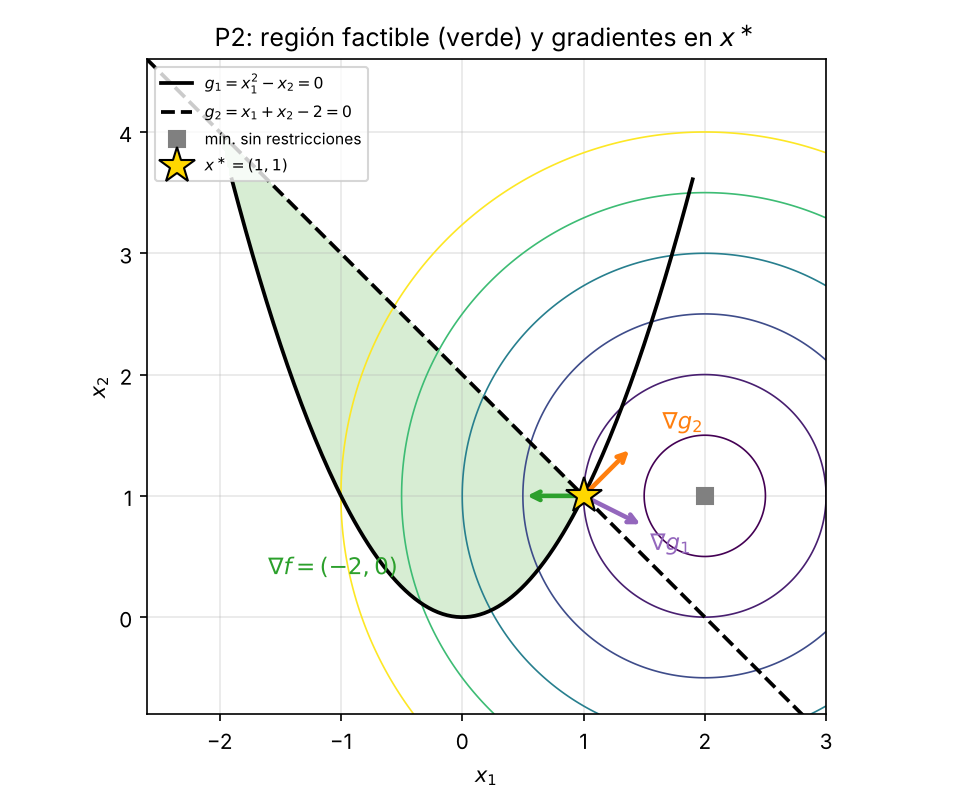
\includegraphics[width=\linewidth]{figs/fig10_kkt_desigualdad.png}
    \end{column}
    \begin{column}{0.47\textwidth}
      \small
      \textbf{Ejemplo P2}
      \[ \min\ (x_1-2)^2+(x_2-1)^2 \]
      \[ \text{s.a.}\quad x_1^2-x_2\le 0,\quad x_1+x_2-2\le 0 \]
      \begin{itemize}
        \item Sin restricciones el mínimo sería $(2,1)$: está \textbf{fuera} de la región verde.
        \item El mínimo con restricciones es $\xs=(1,1)$: está en el \textbf{borde}, en la intersección de las dos restricciones.
        \item Allí $\grad f=(-2,0)\neq 0$: la función \emph{quisiera} seguir bajando hacia la derecha, pero las restricciones se lo impiden.
      \end{itemize}
    \end{column}
  \end{columns}
\end{frame}

\begin{frame}{Mapa de la clase: ¿qué hace cada método con las restricciones?}
  \centering\small
  \begin{tabular}{p{3.5cm}p{4.3cm}p{4.6cm}}
    \toprule
    \textbf{Método} & \textbf{Reemplaza el problema por\dots} & \textbf{Se resuelve con\dots}\\
    \midrule
    \textbf{KKT} & condiciones que cumple el óptimo & ecuaciones (a mano o numérico)\\
    \textbf{Programación cuadrática (QP)} & objetivo cuadrático + restricciones lineales & sistema lineal / conjunto activo\\
    \textbf{Cutting plane} & problema \textbf{lineal} (LP) por linearización & LP repetidos\\
    \textbf{SQP} & un \textbf{QP} en cada iteración (Newton sobre KKT) & QPs repetidos\\
    \textbf{Penalización exterior / interior} & secuencia de problemas \textbf{sin} restricciones & BFGS / Newton (Clase 4)\\
    \bottomrule
  \end{tabular}
  \vspace{0.3cm}

  \normalsize
  Todos se apoyan en lo mismo: \textbf{aproximar localmente} (linealizar, cuadratizar o penalizar) para volver a problemas fáciles.
\end{frame}

\begin{frame}{Problemas de prueba de la clase}
  \small
  \begin{columns}[T]
    \begin{column}{0.5\textwidth}
      \begin{block}{P1 --- una igualdad}
        $\min\ x_1+x_2\quad\text{s.a.}\ x_1^2+x_2^2=2$\\[2pt]
        Solución: $\xs=(-1,-1)$, $f^\ast=-2$, $\lambda^\ast=\tfrac12$.
      \end{block}
      \begin{block}{P2 --- dos desigualdades}
        $\min\ (x_1-2)^2+(x_2-1)^2$\\ s.a.\ $x_1^2\le x_2,\ x_1+x_2\le 2$\\[2pt]
        Solución: $\xs=(1,1)$, $f^\ast=1$, $\mu^\ast=(\tfrac23,\tfrac23)$.
      \end{block}
    \end{column}
    \begin{column}{0.5\textwidth}
      \begin{block}{P3 --- una desigualdad curva}
        $\min\ (x_1-2)^2+(x_2-1)^2\quad\text{s.a.}\ x_1^2+x_2^2\le 1$\\[2pt]
        Solución: $\xs=\tfrac{1}{\sqrt5}(2,1)$, $f^\ast=(\sqrt5-1)^2\approx1.528$, $\mu^\ast=\sqrt5-1$.
      \end{block}
      \begin{block}{P4 --- no convexo}
        Rosenbrock $(1-x_1)^2+100(x_2-x_1^2)^2$ dentro del disco $x_1^2+x_2^2\le1$.\\[2pt]
        Solución: $\xs\approx(0.7864,0.6177)$, $f^\ast\approx0.0457$.
      \end{block}
    \end{column}
  \end{columns}
  \vspace{0.2cm}
  \centering En cada código: parte \textbf{manual} + comparación con \texttt{scipy.optimize} (\texttt{SLSQP}, \texttt{trust-constr}).
\end{frame}
% ============================================================
\section{Condiciones KKT}
% ============================================================

\begin{frame}{Recordatorio: sin restricciones}
  \begin{itemize}
    \item En un mínimo local \textbf{sin restricciones}: $\grad f(\xs)=0$ (si no, podríamos bajar moviéndonos en la dirección $-\grad f$).
    \item Pregunta de hoy: ¿qué \textbf{ecuación equivalente} cumple el mínimo cuando hay restricciones?
  \end{itemize}
  \begin{alertblock}{Estrategia para entenderlo}
    Vamos por pasos: \textbf{(1)} una restricción de igualdad $\to$ multiplicador de Lagrange; \textbf{(2)} una desigualdad $\to$ el multiplicador debe ser $\ge0$; \textbf{(3)} varias restricciones $\to$ condiciones KKT completas.
  \end{alertblock}
  \centering Idea base de todo: \textbf{en un mínimo no se puede mejorar $f$ sin romper alguna restricción.}
\end{frame}

\begin{frame}{Una igualdad: caminar sobre una curva}
  \begin{columns}[T]
    \begin{column}{0.48\textwidth}
      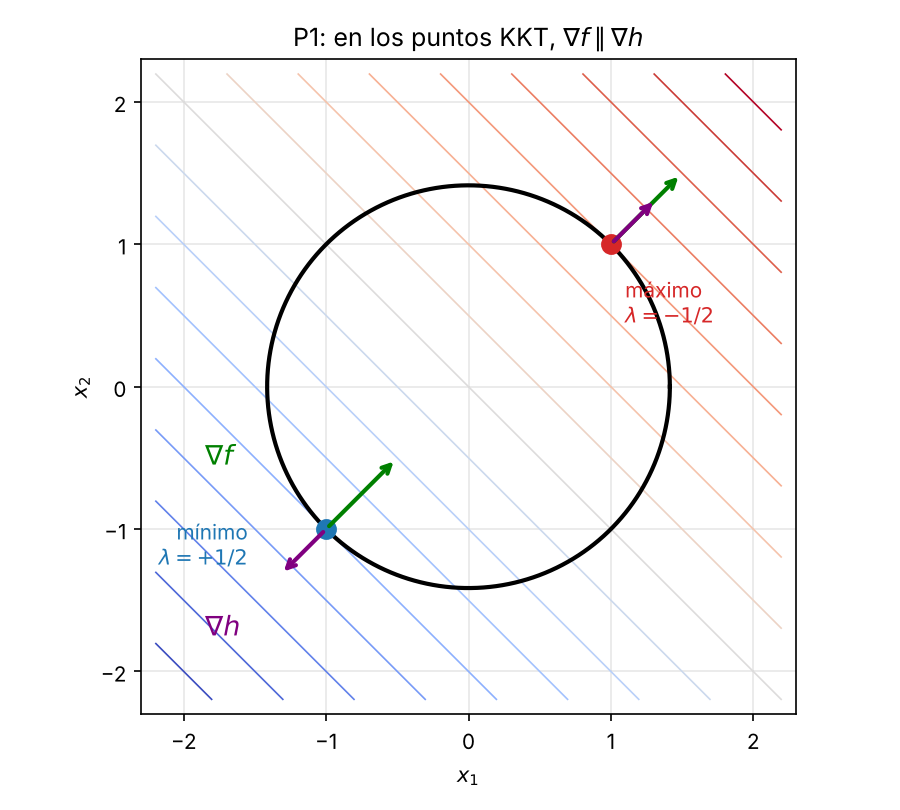
\includegraphics[width=\linewidth]{figs/fig10_kkt_igualdad.png}
    \end{column}
    \begin{column}{0.5\textwidth}
      \small
      \textbf{P1:} $\min\,x_1+x_2$ sobre la circunferencia $x_1^2+x_2^2=2$.
      \begin{itemize}
        \item Solo podemos movernos \textbf{a lo largo de la curva}.
        \item Si $\grad f$ tiene componente a lo largo de la curva, podemos deslizarnos y bajar $f$ $\Rightarrow$ no es mínimo.
        \item En el mínimo, $\grad f$ no tiene componente tangente: es \textbf{perpendicular a la curva}.
        \item Pero $\grad h$ \emph{también} es perpendicular a la curva. Entonces:
      \end{itemize}
      \begin{alertblock}{}
        \centering $\grad f(\xs)\ \parallel\ \grad h(\xs)$
      \end{alertblock}
    \end{column}
  \end{columns}
\end{frame}

\begin{frame}{El multiplicador de Lagrange}
  $\grad f\parallel\grad h$ significa que existe un número $\lambda$ tal que
  \[ \grad f(\xs)+\lambda\,\grad h(\xs)=0,\qquad h(\xs)=0 . \]
  \begin{block}{El Lagrangiano junta todo en una sola función}
    \[ L(x,\lambda)=f(x)+\lambda\,h(x)\qquad\Longrightarrow\qquad
    \grad_x L=0,\quad \grad_\lambda L=h=0 \]
  \end{block}
  \begin{itemize}
    \item Son $n+m$ ecuaciones para $n+m$ incógnitas ($x$ y $\lambda$): un sistema (no lineal) \textbf{sin restricciones}.
    \item Con varias igualdades: $\grad f+\sum_i\lambda_i\grad h_i=0$ ($\grad f$ es combinación lineal de los $\grad h_i$).
    \item \textbf{$\lambda$ puede tener cualquier signo} (en igualdades).
  \end{itemize}
\end{frame}

\begin{frame}{Resolviendo P1 a mano}
  \small
  $L=x_1+x_2+\lambda\,(x_1^2+x_2^2-2)$
  \[ \frac{\partial L}{\partial x_1}=1+2\lambda x_1=0,\qquad
     \frac{\partial L}{\partial x_2}=1+2\lambda x_2=0,\qquad
     x_1^2+x_2^2=2 \]
  De las dos primeras: $x_1=x_2=-\dfrac{1}{2\lambda}$. En la tercera: $\dfrac{2}{4\lambda^2}=2\Rightarrow\lambda^2=\dfrac14$.
  \begin{columns}[T]
    \begin{column}{0.48\textwidth}
      \begin{exampleblock}{$\lambda=+\tfrac12$}
        $x=(-1,-1)$, $f=-2$\\ \textbf{mínimo}
      \end{exampleblock}
    \end{column}
    \begin{column}{0.48\textwidth}
      \begin{alertblock}{$\lambda=-\tfrac12$}
        $x=(1,1)$, $f=+2$\\ \textbf{máximo}
      \end{alertblock}
    \end{column}
  \end{columns}
  \vspace{0.2cm}
  \normalsize
  Las condiciones son \textbf{necesarias pero no suficientes}: el sistema encuentra \emph{todos} los puntos donde $\grad f\parallel\grad h$ (mínimos, máximos y puntos silla). Hay que distinguir después (curvatura, convexidad o comparar valores).
\end{frame}

\begin{frame}{¿Qué significa $\lambda$? El precio sombra}
  Relajemos la restricción: $h(x)=\varepsilon$ en lugar de $h(x)=0$. Sea $f^\ast(\varepsilon)$ el nuevo valor óptimo. Con $L=f+\lambda h$:
  \[ \boxed{\ \frac{d f^\ast}{d\varepsilon}\Big|_{\varepsilon=0}=-\lambda^\ast\ } \]
  \begin{exampleblock}{Comprobación con P1}
    Con $h=\varepsilon$: $x_1^2+x_2^2=2+\varepsilon$, y el mínimo es $f^\ast(\varepsilon)=-\sqrt{4+2\varepsilon}$.
    \[ \frac{df^\ast}{d\varepsilon}\Big|_0=-\frac{1}{\sqrt{4}}=-\frac12=-\lambda^\ast\ \checkmark \]
  \end{exampleblock}
  \begin{itemize}
    \item $\lambda$ mide \textbf{cuánto cambia el óptimo si se afloja la restricción}: es el ``precio'' de la restricción.
    \item Ingeniería: $\lambda$ grande $\Rightarrow$ la restricción que más ``duele'': conviene relajarla.
  \end{itemize}
\end{frame}

\begin{frame}{Desigualdades: activa o inactiva}
  Una restricción $g(x)\le0$ solo puede estar en uno de dos estados en el óptimo $\xs$:
  \begin{columns}[T]
    \begin{column}{0.48\textwidth}
      \begin{block}{Inactiva: $g(\xs)<0$}
        El punto está \textbf{dentro}, con holgura. La restricción ``no se entera'': localmente el problema es como uno sin restricciones.\\[3pt]
        $\Rightarrow$ \textbf{no aporta fuerza}: $\mu=0$.
      \end{block}
    \end{column}
    \begin{column}{0.48\textwidth}
      \begin{block}{Activa: $g(\xs)=0$}
        El punto está \textbf{en el borde}. La restricción se comporta como una igualdad, pero con una diferencia importante\dots\\[3pt]
        $\Rightarrow$ puede aportar fuerza $\mu\ge0$.
      \end{block}
    \end{column}
  \end{columns}
  \vspace{0.3cm}
  \begin{alertblock}{Analogía: una bolita y una valla}
    $f$ es el terreno, la bolita rueda hacia abajo y una valla ($g\le0$) le impide pasar. Si la bolita queda apoyada en la valla, \textbf{la valla la empuja hacia adentro}. Una valla \textbf{solo puede empujar, no jalar}: por eso $\mu\ge0$.
  \end{alertblock}
\end{frame}

\begin{frame}{Por qué $\mu\ge0$: solo se puede empujar hacia adentro}
  \small
  En el borde, una dirección $d$ es \textbf{factible} si no nos saca de la región: $\grad g^\top d\le0$.\\
  En un mínimo \textbf{no existe} una dirección factible que baje $f$:
  \[ \text{no hay } d\ \text{con}\quad \grad f^\top d<0\quad\text{y}\quad \grad g_j^\top d\le 0\ \ (j\ \text{activas}). \]
  Eso equivale (lema de Farkas) a que $-\grad f$ sea combinación \textbf{con coeficientes no negativos} de los $\grad g_j$ activos:
  \[ -\grad f(\xs)=\sum_{j\ \text{activas}}\mu_j\,\grad g_j(\xs),\qquad \mu_j\ge0. \]
  \begin{columns}[T]
    \begin{column}{0.48\textwidth}
      \begin{exampleblock}{Interpretación}
        $-\grad f$ es hacia donde \textbf{quiere ir} la función. Cada $\grad g_j$ apunta hacia \textbf{afuera}. La fuerza total de las vallas ($\mu_j\grad g_j$) compensa exactamente el deseo de ir hacia afuera.
      \end{exampleblock}
    \end{column}
    \begin{column}{0.48\textwidth}
      \begin{alertblock}{Si algún $\mu_j<0$}
        La restricción $j$ estaría ``jalando'' hacia el borde: eso significa que \textbf{soltándola} podríamos mejorar $f$. Esta es la regla que usan los métodos de conjunto activo.
      \end{alertblock}
    \end{column}
  \end{columns}
\end{frame}

\begin{frame}{Geometría en P2: $-\grad f$ dentro del cono de los $\grad g$}
  \begin{columns}[T]
    \begin{column}{0.52\textwidth}
      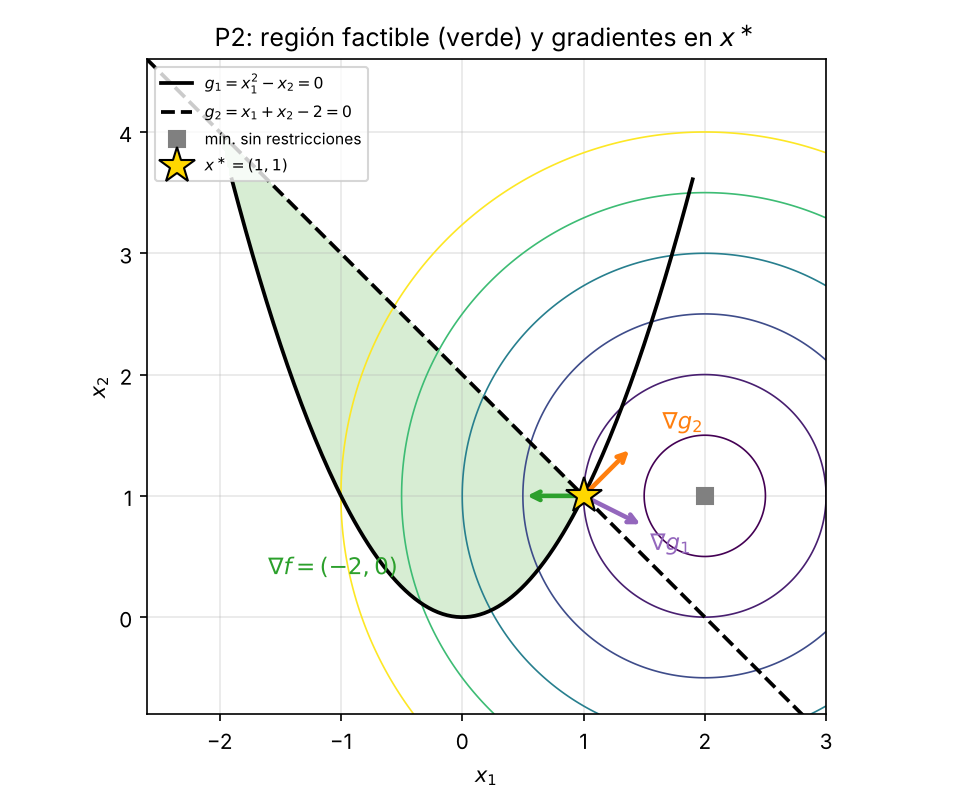
\includegraphics[width=\linewidth]{figs/fig10_kkt_desigualdad.png}
    \end{column}
    \begin{column}{0.46\textwidth}
      \small
      En $\xs=(1,1)$ las dos restricciones están activas:
      \[ \grad f=(-2,0),\quad \grad g_1=(2,-1),\quad \grad g_2=(1,1) \]
      Buscamos $\mu_1,\mu_2\ge0$ tales que $\;-\grad f=\mu_1\grad g_1+\mu_2\grad g_2$:
      \[ \begin{cases} 2\mu_1+\ \mu_2=2\\ -\mu_1+\ \mu_2=0\end{cases}
         \Rightarrow \mu_1=\mu_2=\tfrac23\ \ge 0\ \checkmark \]
      $-\grad f=(2,0)$ cae \textbf{dentro del cono} generado por $\grad g_1$ y $\grad g_2$: no hay forma de bajar $f$ sin salirse de la región.
    \end{column}
  \end{columns}
\end{frame}

\begin{frame}{Las condiciones KKT (Karush--Kuhn--Tucker)}
  Para $\min f(x)$ s.a.\ $h(x)=0,\ g(x)\le0$, si $\xs$ es mínimo local (y las restricciones son ``regulares'') existen $\lambda^\ast,\mu^\ast$ tales que:
  \begin{block}{}
    \begin{tabular}{@{}ll@{}}
      \textbf{1. Estacionariedad:} & $\grad f(\xs)+\sum_i\lambda_i^\ast\grad h_i(\xs)+\sum_j\mu_j^\ast\grad g_j(\xs)=0$\\[3pt]
      \textbf{2. Factibilidad primal:} & $h(\xs)=0,\qquad g(\xs)\le0$\\[3pt]
      \textbf{3. Factibilidad dual:} & $\mu_j^\ast\ge0\quad\forall j$\\[3pt]
      \textbf{4. Complementariedad:} & $\mu_j^\ast\,g_j(\xs)=0\quad\forall j$\\
    \end{tabular}
  \end{block}
  \begin{itemize}
    \item (1) es $\grad_xL=0$. (2) dice que $\xs$ es un punto permitido.
    \item (3) es ``las vallas solo empujan''. (4) dice: \textbf{o la restricción está inactiva ($g<0$) y no actúa ($\mu=0$), o está activa ($g=0$) y puede actuar ($\mu\ge0$)}.
  \end{itemize}
\end{frame}

\begin{frame}{Las cuatro condiciones en lenguaje sencillo}
  \centering\small
  \begin{tabular}{p{3.6cm}p{8.8cm}}
    \toprule
    \textbf{Condición} & \textbf{Qué dice}\\
    \midrule
    Estacionariedad & ``La fuerza que quiere llevarme a un mejor $f$ ($-\grad f$) está equilibrada por las fuerzas de las restricciones''\\[4pt]
    Factibilidad primal & ``Estoy en un punto permitido''\\[4pt]
    Factibilidad dual & ``Las vallas solo empujan hacia adentro (nunca jalan)''\\[4pt]
    Complementariedad & ``Una valla que no estoy tocando no ejerce fuerza''\\
    \bottomrule
  \end{tabular}
  \vspace{0.3cm}

  \normalsize
  \begin{alertblock}{Cómo se usarán hoy}
    \textbf{(a)} verificar si un candidato es óptimo; \textbf{(b)} resolver problemas pequeños por casos; \textbf{(c)} \emph{todos los algoritmos de hoy son formas de resolver las KKT}.
  \end{alertblock}
\end{frame}

\begin{frame}{Uso 1: verificar un candidato en P2}
  Candidato $x=(1,1)$, $\mu=(\tfrac23,\tfrac23)$:
  \begin{center}\small
  \begin{tabular}{lll}
    \toprule
    Condición & Cálculo & ¿Cumple?\\
    \midrule
    1. Estacionariedad & $(-2,0)+\tfrac23(2,-1)+\tfrac23(1,1)=(0,0)$ & sí\\
    2. Factibilidad primal & $g_1=1-1=0\le0,\quad g_2=1+1-2=0\le0$ & sí\\
    3. Factibilidad dual & $\mu=(\tfrac23,\tfrac23)\ge0$ & sí\\
    4. Complementariedad & $\mu_1g_1=0,\ \mu_2g_2=0$ & sí\\
    \bottomrule
  \end{tabular}
  \end{center}
  \begin{alertblock}{Conclusión}
    $(1,1)$ cumple KKT. Como P2 es \textbf{convexo} ($f$ convexa, $g_1,g_2$ convexas), KKT son \textbf{suficientes}: $(1,1)$ es el \textbf{mínimo global}.
  \end{alertblock}
\end{frame}

\begin{frame}{Uso 2: resolver por casos (¿qué restricciones están activas?)}
  Con $p$ desigualdades hay $2^p$ posibilidades de conjunto activo. Para P2: $2^2=4$.
  \begin{center}\small
  \begin{tabular}{llp{4.6cm}c}
    \toprule
    Activas & Solución de estacionariedad & Verificación & ¿KKT?\\
    \midrule
    ninguna & $x=(2,1)$ & $g=(3,1)$: \textbf{infactible} & no\\
    solo $g_1$ & $x=(1.165,1.358)$, $\mu_1=0.72$ & $g_2=0.52>0$: \textbf{infactible} & no\\
    solo $g_2$ & $x=(1.5,0.5)$, $\mu_2=1$ & $g_1=1.75>0$: \textbf{infactible} & no\\
    $g_1,g_2$ & $x=(1,1)$, $\mu=(\tfrac23,\tfrac23)$ & factible, $\mu\ge0$ & \textbf{sí}\\
    $g_1,g_2$ & $x=(-2,4)$, $\mu=(-4.7,-10.7)$ & $\mu<0$ & no\\
    \bottomrule
  \end{tabular}
  \end{center}
  \begin{itemize}
    \item Para cada conjunto activo se resuelve un sistema de \emph{igualdades}; luego se descartan los casos con infactibilidad primal o $\mu<0$.
    \item Funciona para problemas chicos, pero \textbf{$2^p$ crece exponencialmente}: los algoritmos de hoy evitan esta enumeración.
  \end{itemize}
\end{frame}

\begin{frame}{Precio sombra en P2 (comprobación numérica)}
  Relajamos $g_2$: $x_1+x_2\le 2+\varepsilon$ y resolvemos de nuevo (con \texttt{SLSQP}):
  \begin{center}\small
  \begin{tabular}{rr}
    \toprule
    $\varepsilon$ & $f^\ast(\varepsilon)$\\
    \midrule
    $-0.10$ & 1.07296\\
    $-0.01$ & 1.00673\\
    $0$ & 1.00000\\
    $+0.01$ & 0.99340\\
    $+0.10$ & 0.93964\\
    \bottomrule
  \end{tabular}
  \end{center}
  Pendiente numérica en $\varepsilon=0$: $\;\dfrac{f^\ast(0.01)-f^\ast(0)}{0.01}=-0.660,\quad \dfrac{f^\ast(0)-f^\ast(-0.01)}{0.01}\approx-0.673$.
  \begin{alertblock}{Coincide con $-\mu_2^\ast=-\tfrac23\approx-0.667$}
    Cada unidad que se afloje $x_1+x_2\le 2$ reduce el óptimo en $\approx\tfrac23$. Para las desigualdades también: $\;df^\ast/d\varepsilon=-\mu^\ast$.
  \end{alertblock}
\end{frame}

\begin{frame}{Cuidado: cualificación de restricciones}
  KKT son necesarias \textbf{si las restricciones activas son ``regulares''}. La más usada: \textbf{LICQ} --- los gradientes de las restricciones activas ($\grad h_i,\ \grad g_j$ activas) son \textbf{linealmente independientes}.
  \begin{exampleblock}{Contraejemplo}
    $\min\ x\quad\text{s.a.}\quad g(x)=x^2\le 0$.\\
    La única $x$ factible es $0$, así que $\xs=0$ es el mínimo. Pero $\grad f=1$ y $\grad g(0)=0$:
    \[ 1+\mu\cdot 0=0\quad\text{no tiene solución.}\]
    \textbf{El mínimo existe y no cumple KKT}, porque LICQ falla ($\grad g=0$).
  \end{exampleblock}
  \begin{itemize}
    \item En la práctica: si los $\grad g$ activos son dependientes (o se anulan), los multiplicadores pueden no existir o no ser únicos.
    \item Si todas las restricciones son lineales, KKT valen siempre (no se necesita LICQ).
  \end{itemize}
\end{frame}

\begin{frame}{Condiciones de segundo orden: ¿mínimo o máximo?}
  KKT no distinguen mínimos de máximos (P1 tenía ambos). Falta mirar la \textbf{curvatura} --- pero solo \emph{en las direcciones permitidas}:
  \[ d^\top\,\grad^2_{xx}L(\xs,\lambda^\ast,\mu^\ast)\,d>0\quad\text{para toda } d\neq0\ \text{``tangente''},\qquad \grad^2_{xx}L=\grad^2 f+\sum\lambda_i\grad^2h_i+\sum\mu_j\grad^2g_j \]
  \begin{exampleblock}{P1: $\ \grad^2_{xx}L=0+\lambda\cdot 2I=2\lambda I$}
    En $(-1,-1)$: $\lambda=\tfrac12\Rightarrow\grad^2L=I$ definida positiva $\Rightarrow$ \textbf{mínimo}.\\
    En $(1,1)$: $\lambda=-\tfrac12\Rightarrow\grad^2L=-I$ definida negativa $\Rightarrow$ \textbf{máximo}.
  \end{exampleblock}
  \begin{itemize}
    \item Aquí aparece la \textbf{Hessiana del Lagrangiano}, no la de $f$: la curvatura de las restricciones cuenta. (Será clave en SQP.)
    \item En problemas \textbf{convexos} no hace falta: KKT $\Rightarrow$ mínimo global.
  \end{itemize}
\end{frame}

\begin{frame}[fragile]{Código: verificar KKT numéricamente}
\begin{lstlisting}
def residuos_kkt(x, mu, grad, g, Jg):
    est  = np.linalg.norm(grad(x) + Jg(x).T @ mu)  # 1. estacionariedad
    fac  = max(0.0, np.max(g(x)))                  # 2. factibilidad primal
    dual = max(0.0, -np.min(mu))                   # 3. mu >= 0
    comp = np.max(np.abs(mu * g(x)))               # 4. complementariedad
    return est, fac, dual, comp

def multiplicadores_activos(x, grad, g, Jg, tol=1e-8):
    act = np.abs(g(x)) < tol                       # restricciones activas
    mu = np.zeros(len(act))                        # inactivas -> mu = 0
    mu[act] = np.linalg.lstsq(Jg(x)[act].T, -grad(x), rcond=None)[0]
    return mu                                      # grad f + Jg_A' mu = 0
\end{lstlisting}
  \small
  Con la solución de \texttt{SLSQP} en P2: $x=(1,1)$, \ $\mu=(0.6667,\,0.6667)$, residuos $(5\!\times\!10^{-16},\,2\!\times\!10^{-9},\,0,\,1.4\!\times\!10^{-9})$ $\Rightarrow$ KKT cumplidas.
\end{frame}

\begin{frame}{Resumen de KKT}
  \begin{itemize}
    \item \textbf{Igualdad}: $\grad f\parallel\grad h$, con $\lambda$ de cualquier signo.
    \item \textbf{Desigualdad}: la restricción activa empuja hacia adentro: $\mu\ge0$; la inactiva no empuja: $\mu g=0$.
    \item Los \textbf{multiplicadores} son los precios sombra: $df^\ast/d\varepsilon=-\lambda^\ast$ (o $-\mu^\ast$).
    \item KKT son \textbf{necesarias} (con LICQ) y, en problemas \textbf{convexos}, \textbf{suficientes}; en general hay que revisar curvatura (Hessiana del Lagrangiano en el espacio tangente).
  \end{itemize}
  \begin{alertblock}{Puente con el resto de la clase}
    Resolver KKT a mano sirve para problemas chicos. En problemas reales, las KKT forman un \textbf{sistema no lineal con desigualdades} que hay que resolver \emph{numéricamente}. Los cuatro métodos que siguen son distintas maneras de hacerlo: \textbf{QP}, \textbf{cutting plane}, \textbf{SQP} y \textbf{penalización}.
  \end{alertblock}
\end{frame}
% ============================================================
\section{Programación cuadrática (QP)}
% ============================================================

\begin{frame}{¿Qué es un QP y por qué importa?}
  \begin{block}{Problema de programación cuadrática}
    \[ \min_{x\in\R^n}\ \tfrac12 x^\top Hx+c^\top x\quad\text{s.a.}\quad Ax=b,\quad Gx\le h \]
  \end{block}
  \begin{itemize}
    \item \textbf{Objetivo cuadrático} (es el modelo de Newton de la Clase 4) + \textbf{restricciones lineales}.
    \item Aparece directamente: \textbf{mínimos cuadrados con restricciones}, portafolios, control (MPC), SVM\dots
    \item Y, sobre todo, aparece \textbf{como subproblema de SQP}: cada iteración de SQP resuelve un QP. Por eso lo estudiamos primero.
  \end{itemize}
  \begin{alertblock}{Convexidad}
    Si $H$ es \textbf{semidefinida positiva}, el QP es \textbf{convexo}: las KKT son suficientes y todo mínimo local es global. Si $H$ es indefinida, el problema puede ser muy difícil (en general NP-duro). Hoy suponemos $H$ \textbf{definida positiva}.
  \end{alertblock}
\end{frame}

\begin{frame}{Caso 1: solo igualdades $\to$ \textbf{un sistema lineal}}
  $\min\ \tfrac12x^\top Hx+c^\top x\quad\text{s.a.}\quad Ax=b$.\quad Lagrangiano: $L=\tfrac12x^\top Hx+c^\top x+\lambda^\top(Ax-b)$.
  \[ \grad_xL=Hx+c+A^\top\lambda=0,\qquad Ax=b \]
  Son ecuaciones \textbf{lineales} en $(x,\lambda)$. Juntas forman el \textbf{sistema KKT}:
  \[ \boxed{\ \begin{bmatrix} H & A^\top\\ A & 0\end{bmatrix}
     \begin{bmatrix} x\\ \lambda\end{bmatrix}=
     \begin{bmatrix} -c\\ b\end{bmatrix}\ } \]
  \begin{itemize}
    \item \textbf{No hay iteraciones}: se resuelve con \texttt{np.linalg.solve} (un solo paso).
    \item La matriz es simétrica \textbf{indefinida} (``punto silla''); es no singular si $A$ tiene filas independientes y $H$ es definida positiva en el núcleo de $A$.
    \item Con $H=0$ y desigualdades sería un LP; con $A$ vacía se reduce a Newton: $Hx=-c$.
  \end{itemize}
\end{frame}

\begin{frame}{Ejemplo: QP con una igualdad}
  \begin{columns}[T]
    \begin{column}{0.48\textwidth}
      \small
      \[ \min\ (x_1-\tfrac12)^2+2(x_2-\tfrac12)^2\quad\text{s.a.}\ x_1+x_2=3 \]
      $H=\mathrm{diag}(2,4)$, $c=(-1,-2)$, $A=[1\ 1]$, $b=3$:
      \[ \begin{bmatrix}2&0&1\\0&4&1\\1&1&0\end{bmatrix}
         \begin{bmatrix}x_1\\x_2\\\lambda\end{bmatrix}=
         \begin{bmatrix}1\\2\\3\end{bmatrix} \]
      Solución: $x_1=\tfrac{11}{6}$, $x_2=\tfrac76$, $\lambda=-\tfrac83$.\\[4pt]
      La curva de nivel \textbf{es tangente} a la recta en $\xs$: $\grad f\parallel A^\top$.
    \end{column}
    \begin{column}{0.5\textwidth}
      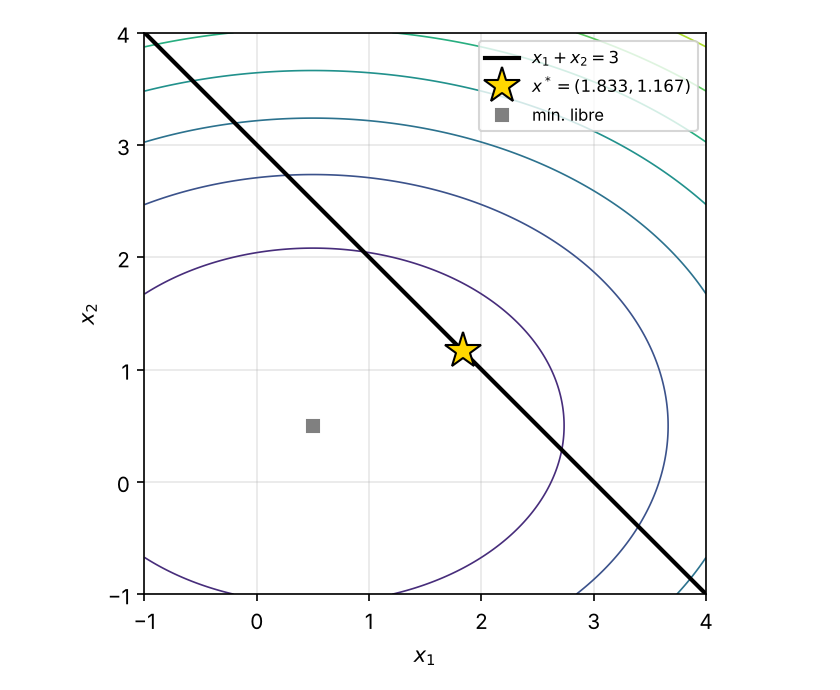
\includegraphics[width=\linewidth]{figs/fig11_qp_igualdad.png}
    \end{column}
  \end{columns}
\end{frame}

\begin{frame}[fragile]{Código: QP de igualdad}
\begin{lstlisting}
def qp_igualdad(H, c, A, b):
    """min 0.5 x'Hx + c'x  s.a. Ax=b  ->  [[H, A'],[A, 0]] [x; lam] = [-c; b]"""
    n, m = H.shape[0], A.shape[0]
    K = np.block([[H, A.T], [A, np.zeros((m, m))]])
    sol = np.linalg.solve(K, np.concatenate([-c, b]))
    return sol[:n], sol[n:]          # x, lambda

# Ejemplo: min x'x  s.a.  x1 + 2 x2 + 3 x3 = 6
H = 2 * np.eye(3); c = np.zeros(3); A = np.array([[1., 2., 3.]]); b = np.array([6.])
x, lam = qp_igualdad(H, c, A, b)
\end{lstlisting}
  \small
  Resultado: $x=\tfrac{6}{14}(1,2,3)=(0.4286,\,0.8571,\,1.2857)$, $\lambda=-0.857$ --- idéntico a \texttt{scipy} (\texttt{SLSQP}).
\end{frame}

\begin{frame}{Caso 2: desigualdades --- ¿cuáles están activas?}
  Si supiéramos qué restricciones están activas en el óptimo, \textbf{el problema sería un QP de igualdad} (un sistema lineal). La dificultad es saberlo.
  \begin{columns}[T]
    \begin{column}{0.48\textwidth}
      \begin{block}{Idea A: probar todas}
        Con $m$ restricciones: $2^m$ combinaciones. Funciona ($m=5\Rightarrow32$ casos y solo 1 cumple KKT), pero crece exponencialmente.
      \end{block}
    \end{column}
    \begin{column}{0.48\textwidth}
      \begin{block}{Idea B: método de conjunto activo}
        \textbf{Adivinar, resolver y corregir}: partir de un conjunto $W$ de restricciones activas, resolver el QP de igualdad, y usar el resultado para \textbf{agregar o soltar} una restricción por iteración.
      \end{block}
    \end{column}
  \end{columns}
  \vspace{0.2cm}
  \centering En la práctica se llega al óptimo en pocos cambios del conjunto $W$.
\end{frame}

\begin{frame}{Método de conjunto activo: las reglas}
  Partimos de un punto \textbf{factible} $x_k$ y un conjunto de restricciones activas $W$ (tratadas como igualdades). Cada iteración:
  \begin{enumerate}
    \item \textbf{Resolver} el QP de igualdad ``en el espacio de $W$'': el paso $p$ que minimiza el modelo con $G_Wp=0$ (un sistema KKT lineal).
    \item \textbf{Si $p\neq0$}: avanzar $x_{k+1}=x_k+\alpha p$ con el \textbf{mayor $\alpha\le1$} que no viole ninguna restricción. Si algo bloquea ($\alpha<1$), \textbf{agregar} esa restricción a $W$.
    \item \textbf{Si $p=0$}: $x_k$ es el mejor punto con $W$ activas. Calcular los \textbf{multiplicadores} $\mu_W$ de las restricciones de $W$.
    \item \textbf{Si todos $\mu\ge0$}: KKT cumplidas $\Rightarrow$ \textbf{óptimo}. Si algún $\mu<0$, esa restricción \textbf{estorba}: \textbf{soltarla} (la más negativa) y repetir.
  \end{enumerate}
  \begin{alertblock}{Paso máximo (restricciones $a_i^\top x\le h_i$ fuera de $W$)}
    \[ \alpha=\min\Bigl\{1,\ \min_{i\notin W,\ a_i^\top p>0}\ \frac{h_i-a_i^\top x}{a_i^\top p}\Bigr\}\qquad \text{(solo frenan las que nos acercan al borde)} \]
  \end{alertblock}
\end{frame}

\begin{frame}{Ejemplo paso a paso: el problema}
  \begin{columns}[T]
    \begin{column}{0.5\textwidth}
      \small
      \[ \min\ (x_1-1)^2+(x_2-2.5)^2 \]
      \vspace{-0.4cm}
      \[ \begin{array}{lll}
        c_1:& x_1-2x_2+2\ge0\\
        c_2:& -x_1-2x_2+6\ge0\\
        c_3:& -x_1+2x_2+2\ge0\\
        c_4:& x_1\ge0\\
        c_5:& x_2\ge0
      \end{array}\]
      \normalsize
      Inicio: $x_0=(2,0)$, con $W_0=\{c_3,c_5\}$ activas (el punto está en la esquina de $c_3$ y $c_5$).\\[3pt]
      \small (En forma $Gx\le h$ se escribe cambiando signos; ver el código.)
    \end{column}
    \begin{column}{0.48\textwidth}
      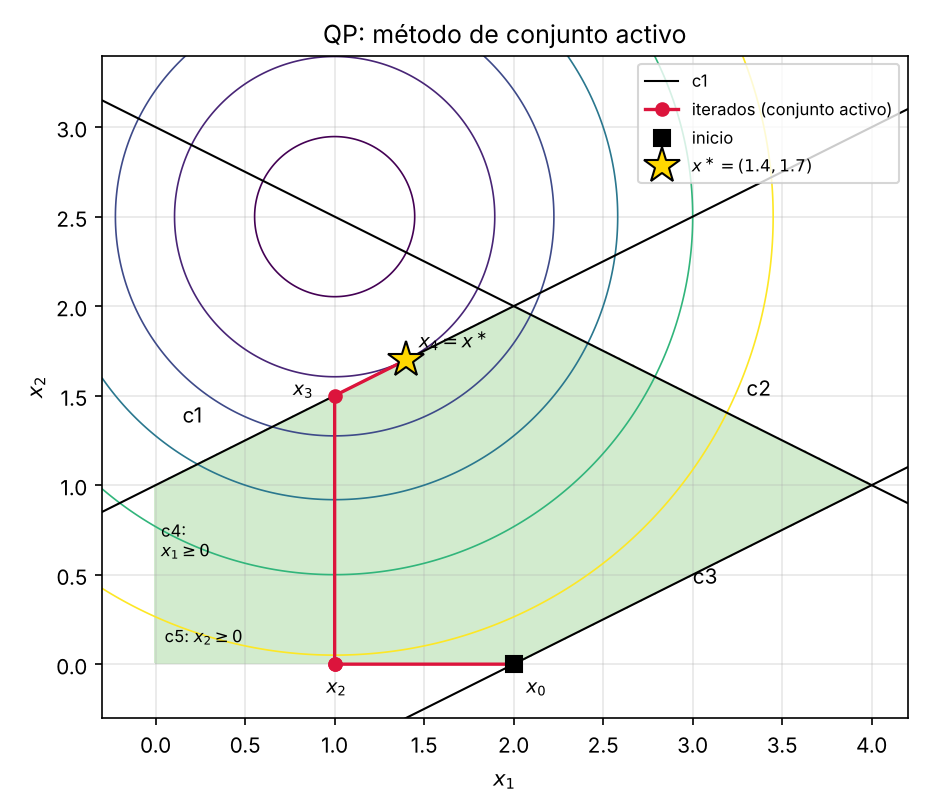
\includegraphics[width=\linewidth]{figs/fig11_qp_conjunto_activo.png}
    \end{column}
  \end{columns}
\end{frame}

\begin{frame}{Ejemplo paso a paso: las iteraciones}
  \small
  \begin{center}
  \begin{tabular}{clllll}
    \toprule
    it. & $x$ & $W$ & paso $p$ y $\alpha$ / multiplicadores & acción\\
    \midrule
    0 & $(2,0)$ & $\{c_3,c_5\}$ & $p=0$;\ $\mu_3=-2,\ \mu_5=-1$ & \textbf{soltar} $c_3$ (más negativo)\\
    1 & $(2,0)$ & $\{c_5\}$ & $p=(-1,0)$, $\alpha=1$ & avanzar a $(1,0)$\\
    2 & $(1,0)$ & $\{c_5\}$ & $p=0$;\ $\mu_5=-5$ & \textbf{soltar} $c_5$\\
    3 & $(1,0)$ & $\emptyset$ & $p=(0,2.5)$, $\alpha=0.6$ & choca con $c_1$: \textbf{agregar} $c_1$\\
    4 & $(1,1.5)$ & $\{c_1\}$ & $p=(0.4,0.2)$, $\alpha=1$ & avanzar a $(1.4,1.7)$\\
    5 & $(1.4,1.7)$ & $\{c_1\}$ & $p=0$;\ $\mu_1=0.8\ge0$ & \textbf{ÓPTIMO}\\
    \bottomrule
  \end{tabular}
  \end{center}
  \normalsize
  \begin{itemize}
    \item $x^\ast=(1.4,\,1.7)$, $f^\ast=0.8$, con \textbf{una sola restricción activa} ($c_1$) y $\mu_1^\ast=0.8$.
    \item Se movió por el \textbf{borde y por el interior}: soltó dos restricciones y agregó una. Total: 6 iteraciones (4 conjuntos activos distintos) frente a $2^5=32$ casos de la enumeración.
  \end{itemize}
\end{frame}

\begin{frame}[fragile]{Código: núcleo del conjunto activo}
\begin{lstlisting}
for k in range(max_iter):
    g = H @ x + c                                   # gradiente del modelo en x
    p = qp_igualdad(H, g, G[W], np.zeros(len(W)))[0] if W else np.linalg.solve(H, -g)
    if np.linalg.norm(p) < tol:                     # x es minimo sobre W
        mu = np.linalg.solve(G[W] @ G[W].T, -G[W] @ g)   # g + G_W' mu = 0
        if np.all(mu >= -tol): break                # KKT cumplidas: OPTIMO
        W.remove(W[int(np.argmin(mu))])             # soltar la mas negativa
    else:
        alpha, blk = 1.0, None                      # paso maximo hasta el borde
        for i in range(G.shape[0]):
            if i not in W and G[i] @ p > 1e-12:
                a_i = (h[i] - G[i] @ x) / (G[i] @ p)
                if a_i < alpha: alpha, blk = a_i, i
        x = x + alpha * p
        if blk is not None: W.append(blk)           # agregar la restriccion bloqueante
\end{lstlisting}
\end{frame}

\begin{frame}{Resultados y comparación con \texttt{scipy}}
  \begin{center}\small
  \begin{tabular}{lcccc}
    \toprule
    Método & $x^\ast$ & $f^\ast$ & iteraciones & Observación\\
    \midrule
    Conjunto activo (manual) & $(1.4,\,1.7)$ & 0.8 & 6 iteraciones & exacto (aritmética lineal)\\
    \texttt{scipy} \texttt{SLSQP} & $(1.4,\,1.7)$ & 0.8 & 3 & SQP con BFGS\\
    \texttt{scipy} \texttt{trust-constr} & $(1.4,\,1.7)$ & 0.8 & 30 & punto interior\\
    \bottomrule
  \end{tabular}
  \end{center}
  \begin{itemize}
    \item Para un QP, el conjunto activo da la solución \textbf{exacta} en un número \textbf{finito} de pasos (no se ``converge'', se \emph{termina}).
    \item La solución coincide con la enumeración de KKT (un solo caso de $2^5$ cumple todo: $S=\{c_1\}$, $\mu_1=0.8$).
  \end{itemize}
  \begin{alertblock}{Observación}
    Los $\mu$ del conjunto activo \textbf{son los multiplicadores de KKT}: el algoritmo \emph{es} una búsqueda guiada del conjunto activo correcto, usando el signo de $\mu$ como brújula.
  \end{alertblock}
\end{frame}

\begin{frame}{Detalles prácticos}
  \begin{itemize}
    \item \textbf{Punto inicial factible}: si no se tiene, se resuelve primero un LP auxiliar (\emph{fase I}) que encuentra un punto factible.
    \item \textbf{$H$ no definida positiva}: el paso $p$ puede no existir o no ser de descenso; se agrega un múltiplo de la identidad o se usan métodos específicos (como en el dogleg de la Clase 4, $B+\lambda I$).
    \item \textbf{Degeneración}: más de $n$ restricciones activas en un punto (ciclado); se usan reglas anti-ciclado.
    \item \textbf{Alternativas}: métodos de \textbf{punto interior} (los usan los solvers modernos para QP grandes) y métodos duales.
  \end{itemize}
  \begin{exampleblock}{Conexión con el miniproyecto}
    Ajustar $y=a\,e^{-bt}+c\,e^{-dt}$ con $b,d>0$ y $b>d$ es un \textbf{problema de mínimos cuadrados con restricciones}. \texttt{scipy.optimize.least\_squares(..., bounds=...)} (métodos \texttt{trf} y \texttt{dogbox}, de tipo trust region) lo resuelve; por dentro aparecen subproblemas cuadráticos con cotas como los de hoy.
  \end{exampleblock}
\end{frame}

\begin{frame}{Resumen de QP}
  \begin{itemize}
    \item QP = objetivo cuadrático + restricciones lineales; convexo si $H\succeq0$.
    \item \textbf{Solo igualdades}: un sistema lineal KKT $\begin{bmatrix}H&A^\top\\A&0\end{bmatrix}\begin{bmatrix}x\\\lambda\end{bmatrix}=\begin{bmatrix}-c\\b\end{bmatrix}$.
    \item \textbf{Con desigualdades}: método de conjunto activo = adivinar $W$, resolver, \textbf{agregar} la restricción que bloquea o \textbf{soltar} la de $\mu<0$.
    \item Termina en un número finito de pasos con la solución exacta.
  \end{itemize}
  \begin{alertblock}{Siguiente pregunta}
    Si el problema real \textbf{no} es un QP (funciones no lineales), ¿cómo usamos esto? Dos caminos: \textbf{linealizar todo} (cutting plane $\to$ LP) o \textbf{cuadratizar} el objetivo y linealizar las restricciones (SQP $\to$ QP).
  \end{alertblock}
\end{frame}
% ============================================================
\section{Cutting plane (planos de corte)}
% ============================================================

\begin{frame}{La idea: reemplazar lo difícil por algo lineal}
  \begin{itemize}
    \item Problema original: $f$ y $g_j$ \textbf{no lineales}. Sabemos resolver muy bien problemas \textbf{lineales} (LP: simplex, puntos interiores).
    \item \textbf{Idea}: aproximar $f$ y $g_j$ por sus \textbf{rectas/planos tangentes} (linearización) y resolver el LP resultante.
    \item Un solo LP no basta: la aproximación es buena solo cerca del punto de tangencia. Entonces se \textbf{agrega un nuevo plano tangente} en cada solución encontrada y se resuelve de nuevo.
  \end{itemize}
  \begin{alertblock}{Por qué se llama ``planos de corte''}
    Cada plano tangente \textbf{corta} una parte de la región donde está permitida la solución del LP, y la va ajustando a la región real. Es el método de \textbf{Kelley} (1960), para problemas \textbf{convexos}.
  \end{alertblock}
\end{frame}

\begin{frame}{Linearizar: el plano tangente es una cota}
  Para $f$ \textbf{convexa}, la tangente en $x_k$ queda \textbf{por debajo} de la función:
  \[ f(x)\ \ge\ f(x_k)+\grad f(x_k)^\top(x-x_k)\quad\forall x. \]
  Igual para cada $g_j$ convexa: $\;g_j(x)\ge g_j(x_k)+\grad g_j(x_k)^\top(x-x_k)$.
  \begin{columns}[T]
    \begin{column}{0.48\textwidth}
      \begin{block}{Consecuencia en las restricciones}
        Si $g_j(x)\le0$, entonces la linearización también es $\le0$. La región \textbf{lineal} $\{g_j(x_k)+\grad g_j(x_k)^\top(x-x_k)\le0\}$ \textbf{contiene} a la región factible real: es una aproximación \textbf{por fuera}.
      \end{block}
    \end{column}
    \begin{column}{0.48\textwidth}
      \begin{block}{Consecuencia en el objetivo}
        El modelo $\max_k\{f(x_k)+\grad f(x_k)^\top(x-x_k)\}$ queda \textbf{por debajo} de $f$: el LP nunca puede ``pasarse'' del óptimo real.
      \end{block}
    \end{column}
  \end{columns}
\end{frame}

\begin{frame}{Cutting plane en 1D: el modelo poliédrico}
  \begin{columns}[T]
    \begin{column}{0.55\textwidth}
      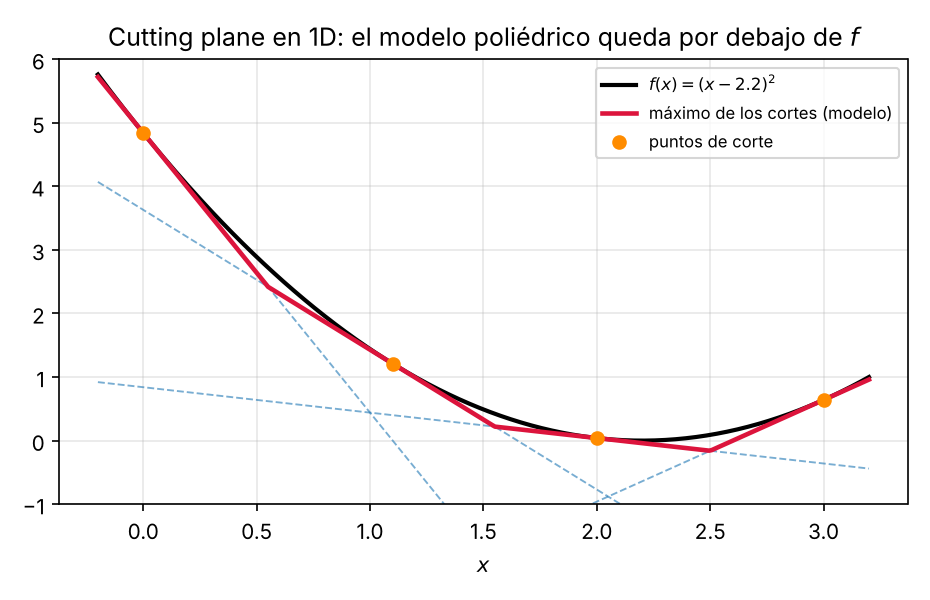
\includegraphics[width=\linewidth]{figs/fig12_cp_1d.png}
    \end{column}
    \begin{column}{0.42\textwidth}
      \small
      \begin{itemize}
        \item Cada punto de corte aporta una \textbf{recta tangente} (líneas punteadas).
        \item El \textbf{modelo} es el máximo de todas las rectas (rojo): una función lineal por tramos \textbf{por debajo} de $f$.
        \item Cuantos más cortes, mejor lo aproxima; los cortes nuevos se agregan \textbf{donde el LP cree que está el mínimo}, así que el modelo se afina justamente donde importa.
      \end{itemize}
    \end{column}
  \end{columns}
\end{frame}

\begin{frame}{El truco del epígrafo}
  Para que \textbf{todo} sea lineal (incluso el objetivo) se introduce una variable $t$:
  \[ \min_x f(x)\quad\Longleftrightarrow\quad \min_{x,t}\ t\quad\text{s.a.}\quad f(x)\le t . \]
  \begin{alertblock}{LP de la iteración $k$ (con los cortes de las iteraciones $0,\dots,k$)}
    \[ \begin{aligned}
    \min_{x,t}\quad & t\\
    \text{s.a.}\quad & f(x_i)+\grad f(x_i)^\top(x-x_i)\le t, && i=0,\dots,k\\
    & g_j(x_i)+\grad g_j(x_i)^\top(x-x_i)\le 0, && i=0,\dots,k,\ \ j=1,\dots,p\\
    & -B\le x\le B &&\text{(caja, para que el LP esté acotado)}
    \end{aligned} \]
  \end{alertblock}
  \begin{itemize}
    \item Es un \textbf{LP} con $n+1$ variables: se resuelve con \texttt{linprog}. Su solución $(x_{k+1},t_{k+1})$ define el siguiente punto de corte.
  \end{itemize}
\end{frame}

\begin{frame}{Algoritmo de cutting plane (Kelley)}
  \begin{enumerate}
    \item Elegir $x_0$ y una caja $[-B,B]^n$ que contenga al óptimo.
    \item \textbf{Agregar cortes} en $x_k$: uno para $f$ y uno por cada $g_j$ (necesita $f,\grad f,g,\grad g$ en $x_k$).
    \item \textbf{Resolver el LP} con todos los cortes acumulados $\to$ $(x_{k+1},t_{k+1})$.
    \item \textbf{Parar} si $x_{k+1}$ es casi factible ($\max g_j\le\text{tol}$) y la brecha $f(x_{k+1})-t_{k+1}\le\text{tol}$. Si no, volver a (2).
  \end{enumerate}
  \begin{exampleblock}{Certificado de optimalidad gratis}
    Como el LP es una relajación, $t_{k+1}\le f^\ast$ es una \textbf{cota inferior} en cada iteración. Si $x_{k+1}$ es factible, $f(x_{k+1})\ge f^\ast$ es una cota superior. La \textbf{brecha} $f(x_{k+1})-t_{k+1}$ dice qué tan cerca estamos --- sin conocer $f^\ast$.
  \end{exampleblock}
  \small Los iterados $x_{k}$ del LP \textbf{pueden ser infactibles} para el problema original (la linearización deja pasar de más): solo al final lo son.
\end{frame}

\begin{frame}{Ejemplo P3 (restricción curva): cómo se cierra el poliedro}
  \centering
  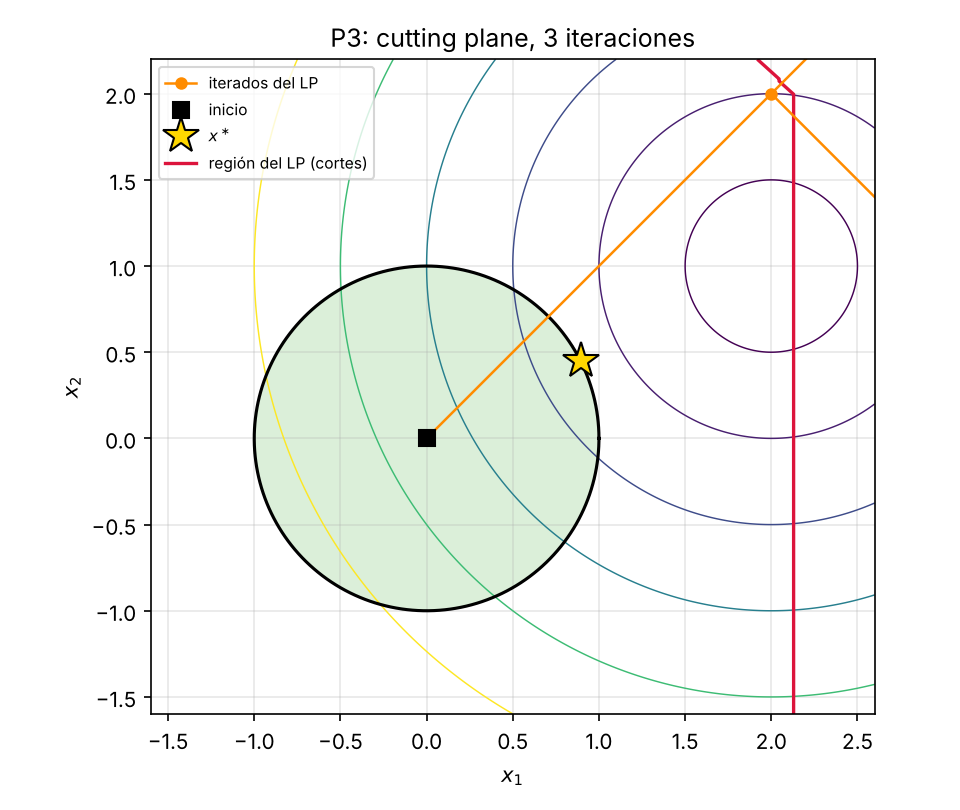
\includegraphics[width=0.31\linewidth]{figs/fig12_cp_P3_k3.png}\hfill
  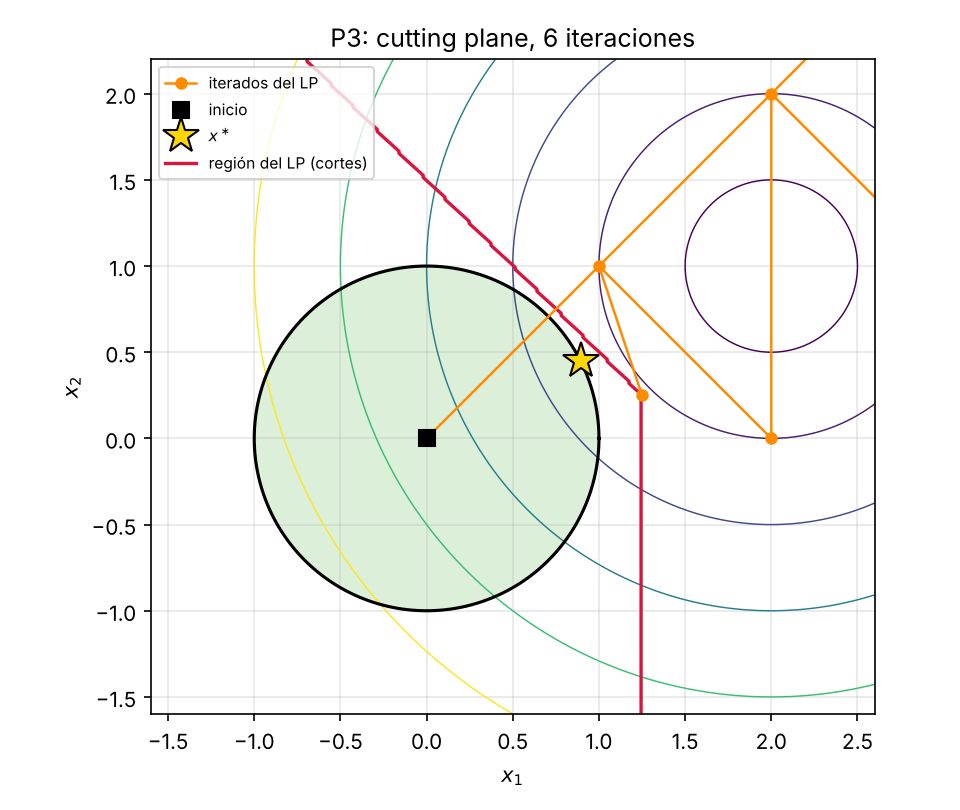
\includegraphics[width=0.31\linewidth]{figs/fig12_cp_P3_k6.png}\hfill
  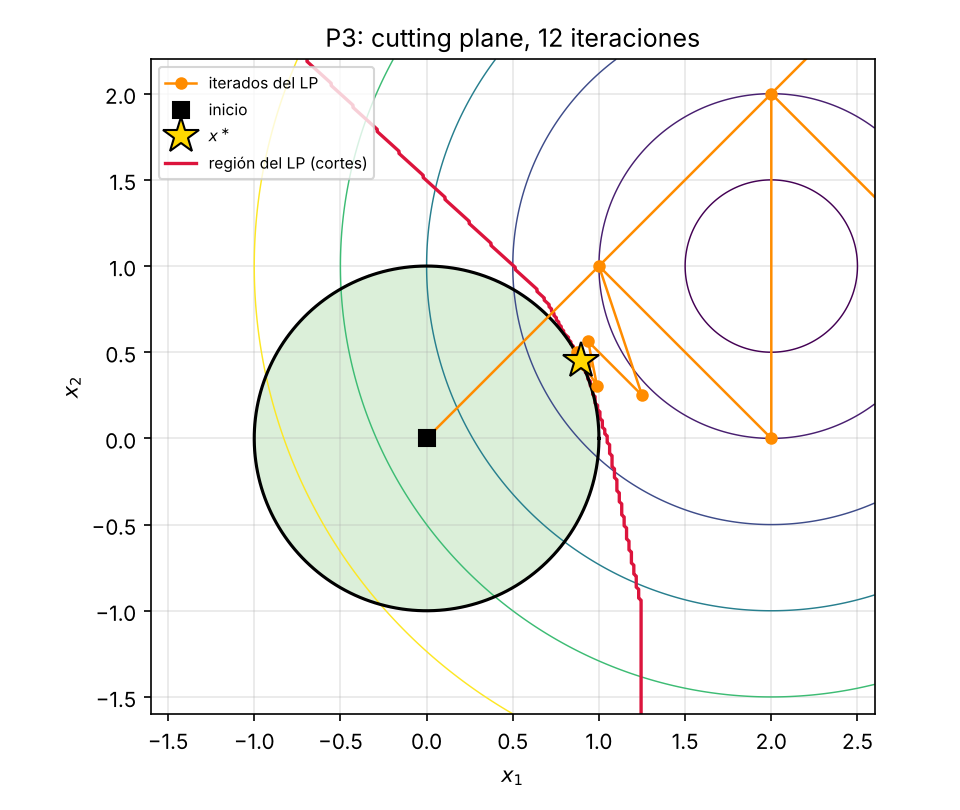
\includegraphics[width=0.31\linewidth]{figs/fig12_cp_P3_k12.png}\\[4pt]
  \small
  Izquierda a derecha: 3, 6 y 12 iteraciones. La curva roja es la \textbf{región del LP} (intersección de los semiplanos de los cortes de $g$): al principio es enorme; luego se \textbf{envuelve} al disco como un polígono circunscrito. Los puntos naranjas (soluciones del LP) \textbf{se acercan a $\xs$ desde afuera} del disco.
\end{frame}

\begin{frame}{P3: convergencia del cutting plane}
  \begin{columns}[T]
    \begin{column}{0.5\textwidth}
      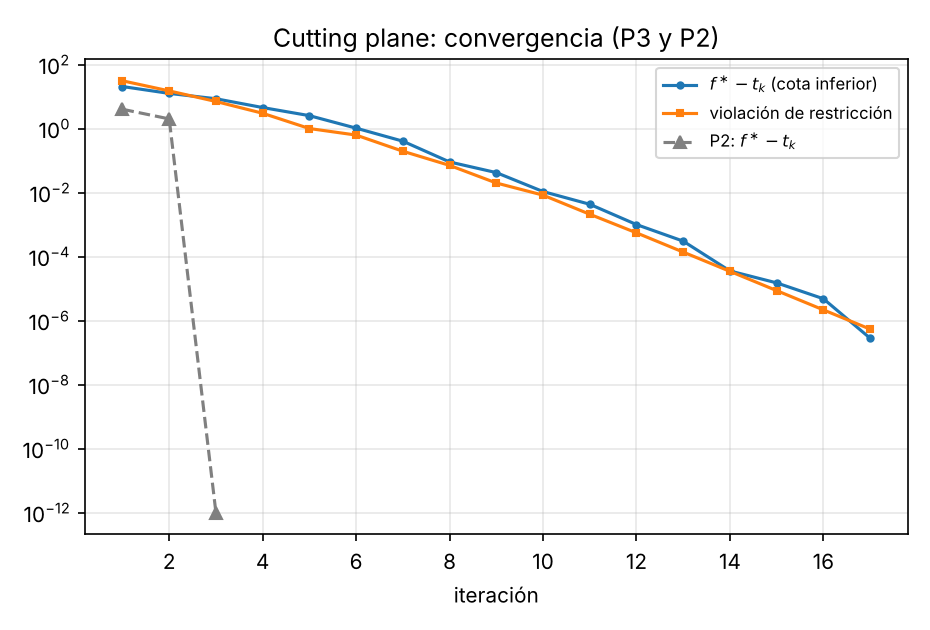
\includegraphics[width=\linewidth]{figs/fig12_cp_conv.png}
    \end{column}
    \begin{column}{0.5\textwidth}
      \scriptsize
      \begin{tabular}{rrrrr}
        \toprule
        $k$ & $x_{k+1}$ & $t_{k+1}$ & $f(x_{k+1})$ & viol.\\
        \midrule
        0 & $(4,\,4)$ & $-19$ & 13 & 31\\
        2 & $(2,\,2)$ & $-7$ & 1 & 7\\
        4 & $(1,\,1)$ & $-1$ & 1 & 1\\
        6 & $(0.94,\,0.56)$ & 1.125 & 1.320 & 0.20\\
        8 & $(0.92,\,0.42)$ & 1.486 & 1.506 & 0.020\\
        9 & $(0.87,\,0.50)$ & 1.517 & 1.525 & 0.008\\
        14 & $(0.895,\,0.446)$ & 1.527849 & 1.527858 & $9\!\times\!10^{-6}$\\
        16 & $(0.8947,\,0.4466)$ & 1.527864 & 1.527864 & $5\!\times\!10^{-7}$\\
        \bottomrule
      \end{tabular}
      \normalsize
      \vspace{3pt}\\
      17 LPs (34 cortes), con $f^\ast=1.527864$: la cota inferior $t_k$ \textbf{sube monótonamente} hacia $f^\ast$.
    \end{column}
  \end{columns}
\end{frame}

\begin{frame}{Contraste: P2 se resuelve en 3 iteraciones}
  \begin{columns}[T]
    \begin{column}{0.5\textwidth}
      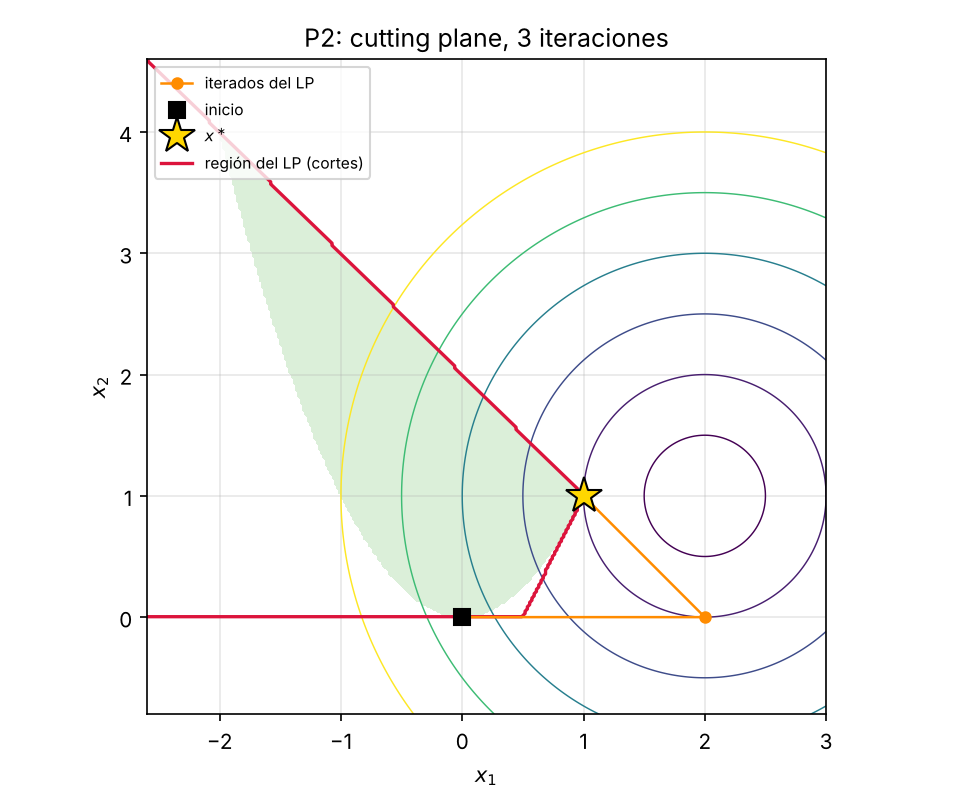
\includegraphics[width=\linewidth]{figs/fig12_cp_P2.png}
    \end{column}
    \begin{column}{0.48\textwidth}
      \small
      \begin{itemize}
        \item En P2 el LP cae \textbf{exactamente} sobre $(1,1)$ en la 2.ª iteración: allí se cruzan la restricción $g_2$ (lineal, su corte es exacto) y la ``punta'' que forman dos tangentes de $f$.
        \item Ese punto es un \textbf{vértice} del poliedro de cortes. En la 3.ª iteración, con las tangentes en $(1,1)$, $t$ sube de $-1$ a $1=f^\ast$ y \textbf{se certifica} el óptimo.
        \item \textbf{No es el caso típico}: cuando el óptimo está sobre una frontera curva (P3), el método tiene que ``circunscribir'' la curva con muchos cortes y converge lento.
      \end{itemize}
    \end{column}
  \end{columns}
\end{frame}

\begin{frame}[fragile]{Código: cutting plane con \texttt{linprog}}
\begin{lstlisting}[basicstyle=\ttfamily\fontsize{7}{8.2}\selectfont,breaklines=false]
def cutting_plane(f, grad, g, Jg, x0, B=4.0, tol=1e-6, max_iter=60):
    x = np.array(x0, float);  A_ub, b_ub = [], []
    for k in range(max_iter):
        fk, gk = f(x), grad(x)
        A_ub.append(np.r_[gk, -1.0]);  b_ub.append(gk @ x - fk)        # corte de f
        for gi, Ji in zip(g(x), Jg(x)):
            A_ub.append(np.r_[Ji, 0.0]);  b_ub.append(Ji @ x - gi)     # corte de g_i
        c = np.zeros(len(x) + 1);  c[-1] = 1.0                         # min t
        res = linprog(c, A_ub=np.array(A_ub), b_ub=np.array(b_ub),
                      bounds=[(-B, B)] * len(x) + [(None, None)], method="highs")
        x, t = res.x[:-1], res.x[-1]
        if max(0.0, np.max(g(x))) < tol and f(x) - t < tol:            # factible y brecha cerrada
            break
    return x
\end{lstlisting}
  \small
  Resultados: P3 $\to$ $x=(0.89471,0.44664)$ con 17 LPs ($\xs=(0.89443,0.44721)$); \texttt{SLSQP}: 17 iteraciones. P2 $\to$ 3 LPs.
\end{frame}

\begin{frame}{Ventajas y límites del cutting plane}
  \begin{columns}[T]
    \begin{column}{0.48\textwidth}
      \begin{block}{Ventajas}
        \begin{itemize}
          \item Muy simple: solo un solver de \textbf{LP} y gradientes.
          \item Maneja \textbf{restricciones no lineales convexas}.
          \item Da \textbf{cotas inferiores} y un certificado de optimalidad.
          \item Funciona con funciones no diferenciables (usando subgradientes).
        \end{itemize}
      \end{block}
    \end{column}
    \begin{column}{0.48\textwidth}
      \begin{block}{Límites}
        \begin{itemize}
          \item \textbf{Lento}: aproxima una curva con segmentos rectos; el costo crece con la dimensión.
          \item \textbf{El LP crece}: cada iteración agrega cortes (memoria y tiempo).
          \item Necesita la \textbf{caja} para acotar el LP; los iterados \textbf{pueden ser infactibles}.
          \item Exige \textbf{convexidad}: sin ella, la tangente ya no es cota y puede cortar al propio óptimo.
        \end{itemize}
      \end{block}
    \end{column}
  \end{columns}
\end{frame}

\begin{frame}{Resumen de cutting plane}
  \begin{itemize}
    \item Convertir el problema en una \textbf{secuencia de LPs} con planos tangentes (cortes) de $f$ y $g_j$, usando el truco del epígrafo.
    \item Los cortes \textbf{nunca eliminan el óptimo} (si el problema es convexo) y el LP da una \textbf{cota inferior} que sube.
    \item Casos con vértice óptimo: muy rápido (P2). Frontera curva: lento (P3, 17 LPs).
  \end{itemize}
  \begin{alertblock}{¿Podemos hacerlo mejor que lineal?}
    Sí: si el modelo del objetivo \textbf{conserva la curvatura} (cuadrático) y solo las restricciones se linearizan, el LP se convierte en un \textbf{QP} y la convergencia pasa de lenta a \textbf{cuadrática}. Eso es la \textbf{programación cuadrática secuencial (SQP)}.
  \end{alertblock}
\end{frame}
% ============================================================
\section{Programación cuadrática secuencial (SQP)}
% ============================================================

\begin{frame}{Recordatorio: Newton = resolver un modelo cuadrático}
  \begin{itemize}
    \item Clase 4, sin restricciones: en $x_k$ se construye el modelo $m(p)=f_k+\grad f_k^\top p+\tfrac12p^\top\grad^2f_k\,p$ y el paso de Newton es su minimizador: $\ \grad^2f_k\,p=-\grad f_k$.
    \item Con restricciones, el equivalente natural es: \textbf{modelo cuadrático del objetivo} + \textbf{restricciones linearizadas}. Eso es exactamente un \textbf{QP}.
  \end{itemize}
  \begin{alertblock}{Idea de SQP}
    \centering En cada iteración: \textbf{resolver un QP} que aproxima el problema en $x_k$, y dar el paso que ese QP propone.
  \end{alertblock}
  \begin{itemize}
    \item Lo bonito: SQP \textbf{no} es un truco inventado; es \textbf{el método de Newton aplicado a las condiciones KKT}. Lo vemos a continuación.
  \end{itemize}
\end{frame}

\begin{frame}{SQP = Newton sobre las condiciones KKT (caso igualdades)}
  \small
  Para $\min f$ s.a.\ $h(x)=0$ las KKT son un sistema de $n+m$ ecuaciones:
  \[ F(x,\lambda)=\begin{bmatrix}\grad f(x)+J_h(x)^\top\lambda\\ h(x)\end{bmatrix}=0 \qquad (J_h=\text{jacobiana de }h) \]
  Newton para $F=0$ (con $W=\grad^2_{xx}L$ la Hessiana del Lagrangiano):
  \[ \begin{bmatrix}W&J_h^\top\\J_h&0\end{bmatrix}\begin{bmatrix}p\\\Delta\lambda\end{bmatrix}=-\begin{bmatrix}\grad_xL\\h\end{bmatrix}
     \ \Longleftrightarrow\
     \boxed{\begin{bmatrix}W&J_h^\top\\J_h&0\end{bmatrix}\begin{bmatrix}p\\\lambda_{+}\end{bmatrix}=\begin{bmatrix}-\grad f\\-h\end{bmatrix}},\quad \lambda_+=\lambda+\Delta\lambda \]
  \begin{alertblock}{¡Es el sistema KKT de un QP!}
    \[ \min_p\ \grad f^\top p+\tfrac12p^\top Wp\qquad\text{s.a.}\qquad J_h\,p+h=0 \]
    (compare con la diapositiva ``QP de igualdad'': $H\to W$, $c\to\grad f$, $A\to J_h$, $b\to-h$.) Resolver el QP \textbf{es} dar un paso de Newton sobre KKT, y su multiplicador $\lambda_+$ es la nueva estimación de $\lambda$.
  \end{alertblock}
\end{frame}

\begin{frame}{El subproblema QP completo (con desigualdades)}
  En $x_k$ (con multiplicadores actuales $\lambda_k,\mu_k$):
  \begin{block}{}
    \[ \begin{aligned}
    \min_{p}\quad & \grad f(x_k)^\top p+\tfrac12\,p^\top W_k\,p\\
    \text{s.a.}\quad & h(x_k)+J_h(x_k)\,p=0\\
    & g(x_k)+J_g(x_k)\,p\le0
    \end{aligned}\qquad W_k=\grad^2f_k+\sum_i\lambda_i\grad^2h_i+\sum_j\mu_j\grad^2g_j \]
  \end{block}
  \begin{itemize}
    \item Las restricciones se \textbf{linearizan} (como en cutting plane); el objetivo se \textbf{cuadratiza} (como en Newton). Se resuelve con el método de conjunto activo.
    \item Del QP salen el paso $p_k$ \textbf{y} los multiplicadores $\lambda_{k+1},\mu_{k+1}$ (\textbf{gratis}, son los de KKT del QP).
    \item El conjunto activo del QP \textbf{predice} qué restricciones estarán activas en el óptimo real.
  \end{itemize}
\end{frame}

\begin{frame}{¿Por qué $W$ es la Hessiana del Lagrangiano y no la de $f$?}
  \begin{columns}[T]
    \begin{column}{0.54\textwidth}
      \small
      \textbf{P1:} $f=x_1+x_2$ es \emph{lineal}: $\grad^2f=0$.
      \begin{itemize}
        \item Si usáramos $W=\grad^2f=0$, el QP sería un \textbf{LP} sobre la restricción linearizada (una recta): \textbf{sin mínimo} (se escapa al infinito).
        \item Con $W=\grad^2_{xx}L=\lambda\cdot2I$, el QP ``ve'' la \textbf{curvatura de la circunferencia}: tiene mínimo y apunta bien al óptimo.
      \end{itemize}
      \begin{alertblock}{Moraleja}
        La curvatura de las restricciones \textbf{también cuenta} en el óptimo (ya lo vimos en las condiciones de 2.º orden). Por eso SQP modela el \textbf{Lagrangiano}, no solo $f$.
      \end{alertblock}
    \end{column}
    \begin{column}{0.44\textwidth}
      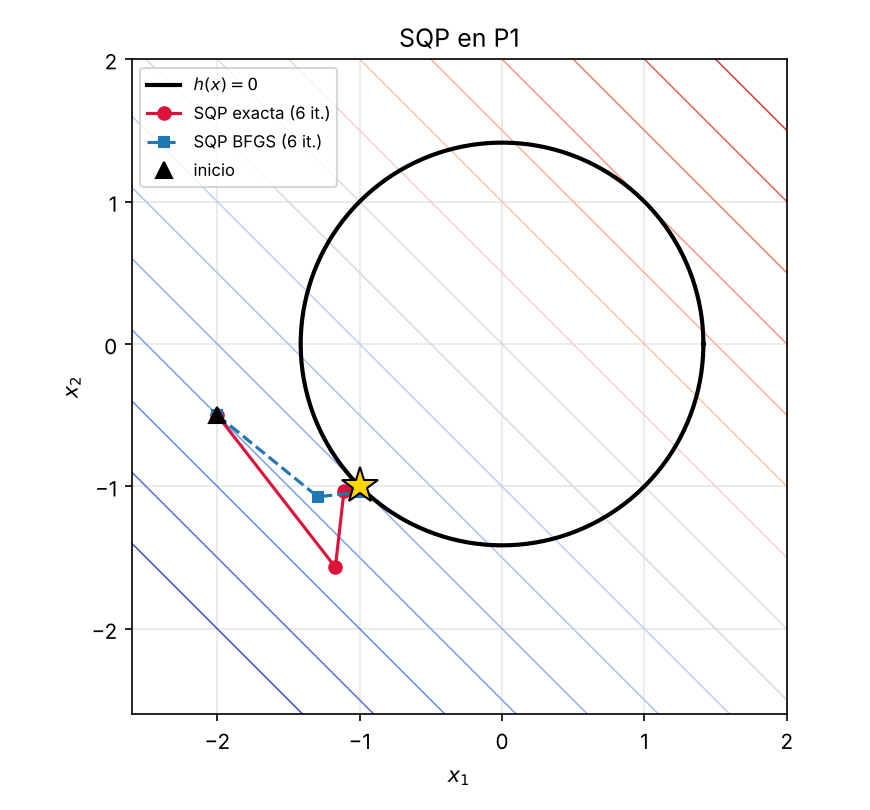
\includegraphics[width=\linewidth]{figs/fig13_sqp_P1.png}
    \end{column}
  \end{columns}
\end{frame}

\begin{frame}{Algoritmo SQP básico}
  \begin{enumerate}
    \item Dado $x_k$ y multiplicadores $\lambda_k,\mu_k$: calcular $f,\grad f,h,J_h,g,J_g$ y $W_k$ (exacta o aproximada).
    \item \textbf{Resolver el QP} $\to$ paso $p_k$ y nuevos multiplicadores $\hat\lambda,\hat\mu$.
    \item \textbf{Elegir $\alpha_k\in(0,1]$} por búsqueda lineal sobre una \textbf{función de mérito} (siguiente diapositiva).
    \item Actualizar: $x_{k+1}=x_k+\alpha_kp_k$, $\ \lambda_{k+1}=\lambda_k+\alpha_k(\hat\lambda-\lambda_k)$, igual para $\mu$.
    \item Parar si $\max\bigl(\norm{\grad_xL}_\infty,\ \text{violación},\ \max|\mu_jg_j|\bigr)<\text{tol}$ (\textbf{el criterio es KKT}).
  \end{enumerate}
  \begin{exampleblock}{Comparación con las clases anteriores}
    Es el \textbf{mismo esqueleto} de Newton con line search (Clase 4): un paso de un modelo cuadrático + control del tamaño del paso. La novedad: el modelo es un QP con restricciones y hace falta una función de mérito para decidir si el paso mejora.
  \end{exampleblock}
\end{frame}

\begin{frame}{Globalización: la función de mérito $\ell_1$}
  \begin{itemize}
    \item Lejos de la solución, Newton puede dar pasos que \textbf{bajan} $f$ pero \textbf{violan} más las restricciones (o al revés). Sin restricciones, el criterio era ``$f$ baja''. Con restricciones hay \textbf{dos objetivos en conflicto}.
    \item Solución: una función que mide \textbf{ambos}:
  \end{itemize}
  \[ \phi(x;\nu)=f(x)+\nu\Bigl(\sum_i|h_i(x)|+\sum_j\max\{0,g_j(x)\}\Bigr),\qquad \nu>0 \]
  \begin{columns}[T]
    \begin{column}{0.5\textwidth}
      \begin{block}{Búsqueda lineal (Armijo)}
        Aceptar $\alpha$ si
        \[ \phi(x+\alpha p)\le\phi(x)+\eta\,\alpha\,D, \]
        con $\eta=10^{-4}$, $\ D=\grad f^\top p-\nu\cdot\text{viol}(x)$, y retroceder $\alpha\leftarrow\alpha/2$ si no.
      \end{block}
    \end{column}
    \begin{column}{0.48\textwidth}
      \begin{block}{Elección de $\nu$}
        Debe ser \textbf{mayor que los multiplicadores} ($\nu>\norm{\lambda}_\infty,\ \max\mu_j$): así $\phi$ es una \textbf{penalización exacta} (su mínimo \emph{es} el de la restricción) y el paso $p$ de SQP es \textbf{dirección de descenso} de $\phi$.
      \end{block}
    \end{column}
  \end{columns}
\end{frame}

\begin{frame}{Hessiana exacta o BFGS}
  \begin{columns}[T]
    \begin{column}{0.48\textwidth}
      \begin{block}{Hessiana exacta de $L$}
        Convergencia \textbf{cuadrática}, pero necesita segundas derivadas de $f$ \textbf{y de las restricciones}. Puede ser indefinida $\Rightarrow$ se la corrige (sumar $\tau I$) para que el QP sea convexo.
      \end{block}
    \end{column}
    \begin{column}{0.48\textwidth}
      \begin{block}{Aproximación BFGS de $W$}
        Como en la Clase 4, se actualiza con $s=x_{k+1}-x_k$ y $y=\grad_xL(x_{k+1},\lambda_{+})-\grad_xL(x_k,\lambda_{+})$. Convergencia \textbf{superlineal}, \textbf{solo primeras derivadas}.
      \end{block}
    \end{column}
  \end{columns}
  \vspace{0.2cm}
  \begin{alertblock}{Amortiguamiento de Powell}
    La Hessiana del Lagrangiano \textbf{no} es definida positiva en general, así que $s^\top y$ puede ser $\le0$ y romper BFGS. Powell reemplaza $y$ por $r=\theta y+(1-\theta)Bs$ (con $\theta\in[0,1]$ elegido para que $s^\top r\ge0.2\,s^\top Bs$), que \textbf{mantiene $B$ definida positiva}.
  \end{alertblock}
\end{frame}

\begin{frame}{Ejemplo P1: iteraciones de SQP (Hessiana exacta)}
  \begin{columns}[T]
    \begin{column}{0.5\textwidth}
      \small
      $x_0=(-2,\,-0.5)$, \ $\lambda_0$ por mínimos cuadrados:
      \begin{center}\scriptsize
      \begin{tabular}{rrrr}
        \toprule
        $k$ & $x_k$ & $f(x_k)$ & viol.\\
        \midrule
        0 & $(-2,\,-0.5)$ & $-2.5$ & 2.25\\
        1 & $(-1.1706,\,-1.5676)$ & $-2.738$ & 1.83\\
        2 & $(-1.1097,\,-1.0301)$ & $-2.140$ & 0.29\\
        3 & $(-0.9988,\,-1.0075)$ & $-2.0064$ & $1.3\!\times\!10^{-2}$\\
        4 & $(-1.00006,\,-0.99997)$ & $-2.00003$ & $5.8\!\times\!10^{-5}$\\
        5 & $(-1,\,-1)$ & $-2$ & $4\!\times\!10^{-9}$\\
        \bottomrule
      \end{tabular}
      \end{center}
      \normalsize
      Converge a $\xs=(-1,-1)$, $\lambda^\ast=0.5$.
    \end{column}
    \begin{column}{0.46\textwidth}
      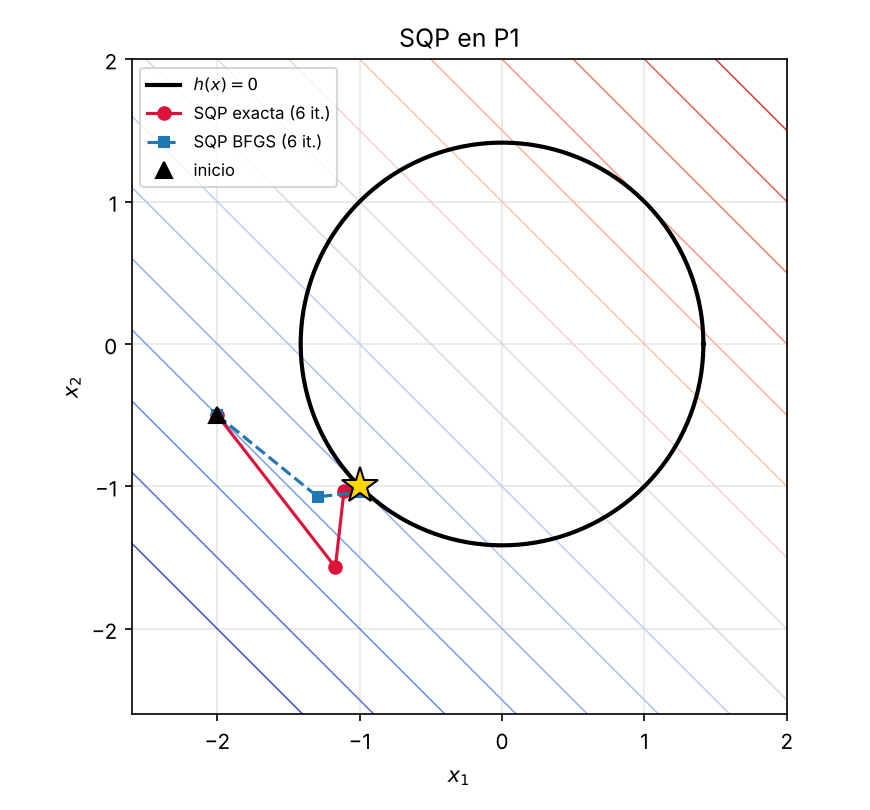
\includegraphics[width=\linewidth]{figs/fig13_sqp_P1.png}\\
      \scriptsize Ambas versiones (exacta y BFGS) llegan en 6 iteraciones; el punto inicial es infactible y las iteraciones \textbf{van acercándose a la circunferencia} mientras $f$ sube hacia $-2$.
    \end{column}
  \end{columns}
\end{frame}

\begin{frame}{Tasa de convergencia: cuadrática vs. superlineal}
  \begin{columns}[T]
    \begin{column}{0.56\textwidth}
      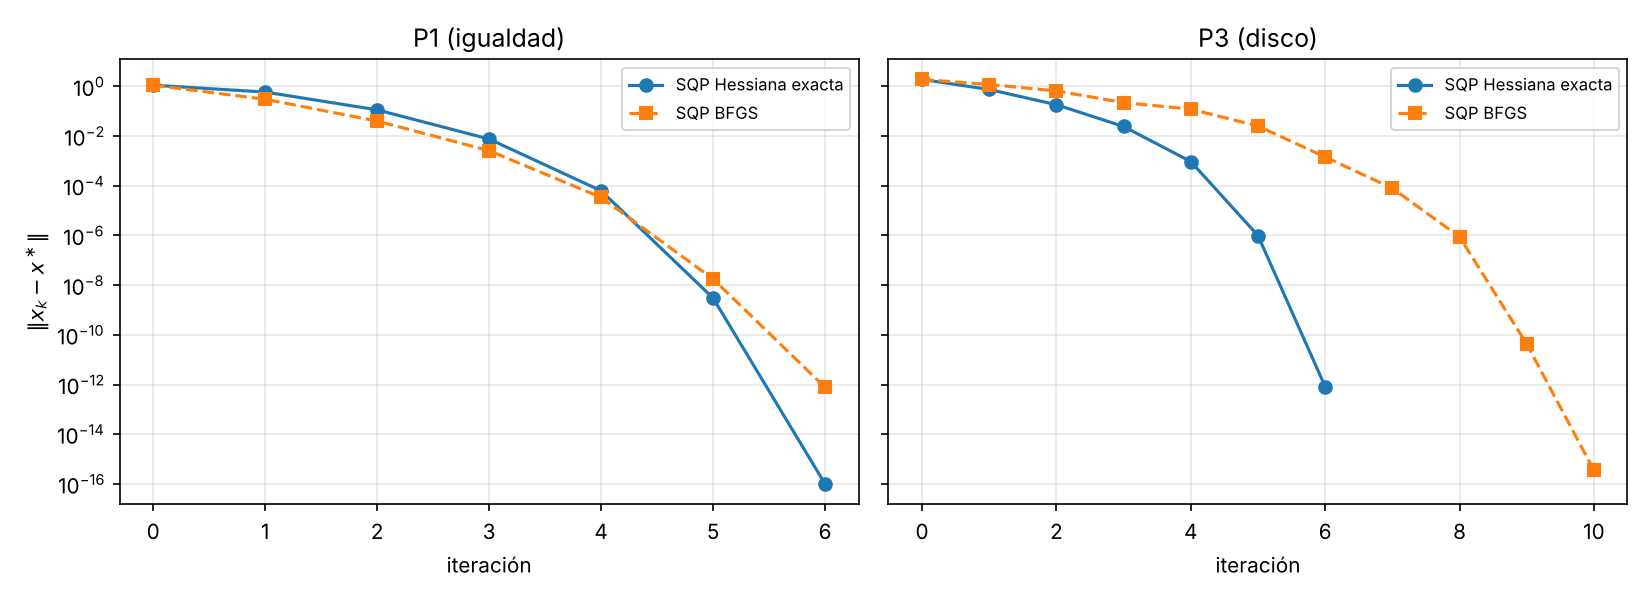
\includegraphics[width=\linewidth]{figs/fig13_sqp_conv.png}
    \end{column}
    \begin{column}{0.42\textwidth}
      \small
      Error $\norm{x_k-\xs}$ en P3 (disco):
      \begin{center}\scriptsize
      \begin{tabular}{rll}
        \toprule
        $k$ & exacta & BFGS\\
        \midrule
        1 & $7.5\!\times\!10^{-1}$ & $1.2$\\
        2 & $1.8\!\times\!10^{-1}$ & $6.6\!\times\!10^{-1}$\\
        3 & $2.4\!\times\!10^{-2}$ & $2.2\!\times\!10^{-1}$\\
        4 & $9.4\!\times\!10^{-4}$ & $1.2\!\times\!10^{-1}$\\
        5 & $9.9\!\times\!10^{-7}$ & $2.5\!\times\!10^{-2}$\\
        6 & $8.3\!\times\!10^{-13}$ & $1.4\!\times\!10^{-3}$\\
        \bottomrule
      \end{tabular}
      \end{center}
      \normalsize
      \textbf{Exacta}: el error se \emph{eleva al cuadrado} ($10^{-4}\to10^{-7}\to10^{-13}$). \textbf{BFGS}: más iteraciones pero cada una más barata.
    \end{column}
  \end{columns}
\end{frame}

\begin{frame}{Ejemplo P2: SQP y el conjunto activo del QP}
  \begin{columns}[T]
    \begin{column}{0.52\textwidth}
      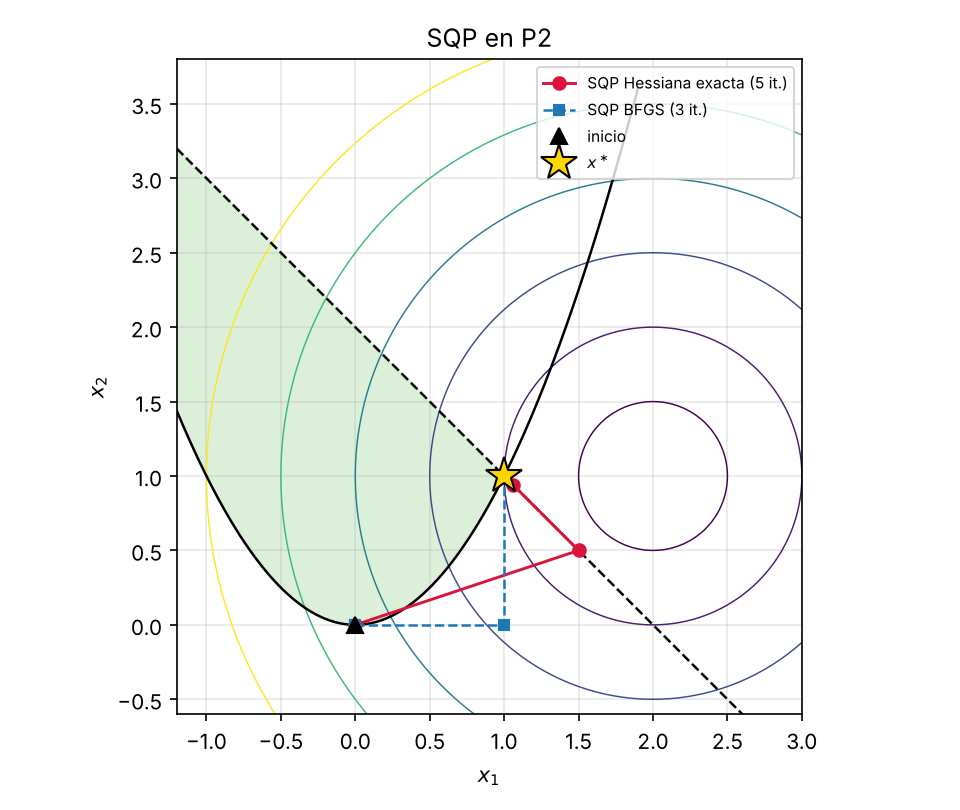
\includegraphics[width=\linewidth]{figs/fig13_sqp_P2.png}
    \end{column}
    \begin{column}{0.46\textwidth}
      \scriptsize
      \begin{tabular}{rllc}
        \toprule
        $k$ & $x_k$ & error & activas en el QP\\
        \midrule
        0 & $(0,\,0)$ & 1.41 & $g_2$\\
        1 & $(1.5,\,0.5)$ & 0.71 & $g_1,g_2$\\
        2 & $(1.0625,\,0.9375)$ & $8.8\!\times\!10^{-2}$ & $g_1,g_2$\\
        3 & $(1.00125,\,0.99875)$ & $1.8\!\times\!10^{-3}$ & $g_1,g_2$\\
        4 & $(1.000001,\,0.999999)$ & $1.4\!\times\!10^{-6}$ & $g_1,g_2$\\
        5 & $(1,\,1)$ & $\sim10^{-12}$ & --\\
        \bottomrule
      \end{tabular}
      \normalsize
      \begin{itemize}
        \item $\alpha=1$ en todas las iteraciones.
        \item Desde la 1.ª iteración el QP \textbf{identifica las dos restricciones activas}; luego es Newton puro sobre KKT.
        \item Multiplicadores finales: $\mu=(\tfrac23,\tfrac23)$ \checkmark{}.
      \end{itemize}
    \end{column}
  \end{columns}
\end{frame}

\begin{frame}[fragile]{Código: el QP por enumeración de conjuntos activos}
\begin{lstlisting}[basicstyle=\ttfamily\fontsize{7}{8.2}\selectfont,breaklines=false]
def resolver_qp(W, gf, Aeq, ceq, Ain, cin, tol=1e-9):
    """min gf'p + 0.5 p'Wp  s.a. Aeq p + ceq = 0,  Ain p + cin <= 0."""
    n, me, mi = len(gf), len(ceq), len(cin)
    for r in range(mi + 1):                       # prueba subconjuntos S de desigualdades activas
        for S in itertools.combinations(range(mi), r):
            S = list(S)
            A = np.vstack([Aeq, Ain[S]]);  rhs = np.concatenate([-ceq, -cin[S]])
            K = np.block([[W, A.T], [A, np.zeros((len(rhs), len(rhs)))]])
            sol = np.linalg.solve(K, np.concatenate([-gf, rhs]))   # sistema KKT de igualdad
            p, nu = sol[:n], sol[n:]
            lam, mu_S = nu[:me], nu[me:]
            if mi and np.any(Ain @ p + cin > tol):  continue       # viola otra desigualdad
            if len(S) and np.any(mu_S < -tol):      continue       # mu < 0: no es KKT
            mu = np.zeros(mi);  mu[S] = mu_S
            return p, lam, mu, S
\end{lstlisting}
  \small Exacto y claro para pocas desigualdades; en la práctica se usa el conjunto activo de la sección de QP.
\end{frame}

\begin{frame}[fragile]{Código: bucle principal de SQP}
\begin{lstlisting}[basicstyle=\ttfamily\fontsize{7}{8.2}\selectfont,breaklines=false]
def sqp(prob, x0, modo="exacta", tol=1e-9, max_iter=50):
    x = np.array(x0, float);  B = np.eye(len(x));  nu_pen = 1.0
    lam = np.linalg.lstsq(Jh(x).T, -grad(x), rcond=None)[0] if me else np.zeros(0);  mu = np.zeros(mi)
    for k in range(max_iter):
        kkt = max(np.max(np.abs(gradL(x, lam, mu))), viol(x), np.max(np.abs(mu * g(x))))
        if kkt < tol:  break                                   # criterio de parada: KKT
        W = hessL(x, lam, mu) if modo == "exacta" else B       # Hessiana del Lagrangiano
        W = W + max(0.0, 1e-3 - np.linalg.eigvalsh(W).min()) * np.eye(len(x))   # W definida positiva
        p, lam_n, mu_n, S = resolver_qp(W, grad(x), Jh(x), h(x), Jg(x), g(x))   # QP
        nu_pen = max(nu_pen, 1.1 * np.max(np.abs(np.r_[lam_n, mu_n])) + 1e-3)   # penalidad de merito
        D = grad(x) @ p - nu_pen * viol(x);  alpha = 1.0
        while phi(x + alpha*p, nu_pen) > phi(x, nu_pen) + 1e-4*alpha*D:  alpha /= 2   # Armijo
        x_new = x + alpha * p
        lam, mu = lam + alpha*(lam_n - lam), mu + alpha*(mu_n - mu)
        if modo == "bfgs": B = bfgs_powell(B, x_new - x, gradL(x_new, lam, mu) - gradL(x, lam, mu))
        x = x_new
    return x, lam, mu
\end{lstlisting}
  \small (Versión resumida; el archivo completo está en \texttt{scripts/13\_sqp.py}.)
\end{frame}

\begin{frame}{Resultados: P3 (convexo) y P4 (Rosenbrock en el disco, no convexo)}
  \scriptsize
  \begin{columns}[T]
    \begin{column}{0.49\textwidth}
      \textbf{P3} --- $\xs=(0.8944,0.4472)$
      \begin{center}
      \begin{tabular}{lrrrr}
        \toprule
        Método & iter. & eval.\ $f$ & eval.\ $\grad f$ & error\\
        \midrule
        SQP exacta & 6 & 19 & 13 & $<10^{-12}$\\
        SQP BFGS & 7 & 30 & 29 & $10^{-16}$\\
        \texttt{SLSQP} & 9 & 11 & 9 & $3\!\times\!10^{-15}$\\
        \bottomrule
      \end{tabular}
      \end{center}
    \end{column}
    \begin{column}{0.49\textwidth}
      \textbf{P4} --- $\xs=(0.7864,0.6177)$, $f^\ast=0.0457$
      \begin{center}
      \begin{tabular}{lrrrr}
        \toprule
        Método & iter. & eval.\ $f$ & eval.\ $\grad f$ & error\\
        \midrule
        SQP exacta & 6 & 41 & 13 & $5\!\times\!10^{-9}$\\
        SQP BFGS & 22 & 97 & 89 & $5\!\times\!10^{-9}$\\
        \texttt{SLSQP} & 17 & 23 & 17 & $5\!\times\!10^{-9}$\\
        \bottomrule
      \end{tabular}
      \end{center}
    \end{column}
  \end{columns}
  \normalsize
  \vspace{0.2cm}
  \begin{itemize}
    \item El SQP manual coincide con \texttt{scipy SLSQP} (que \emph{es} un SQP con BFGS y función de mérito $\ell_1$) en \textbf{la solución y en el orden de magnitud de iteraciones}.
    \item P4 es \textbf{no convexo} (Rosenbrock): SQP sigue funcionando porque solo necesita \textbf{puntos KKT} locales; cutting plane \textbf{no} aplicaría.
    \item Conteos aproximados (cada evaluación del mérito $\phi$ cuenta como una evaluación de $f$).
  \end{itemize}
\end{frame}

\begin{frame}{Dos advertencias honestas}
  \begin{alertblock}{SQP converge a \emph{puntos KKT}, no necesariamente al mínimo}
    En P1, $(1,1)$ es un \textbf{máximo} que también cumple KKT. Partiendo de $x_0=(1.5,1)$ (cerca de él) nuestro SQP llega al mínimo, pero tarda \textbf{49 iteraciones} con Hessiana exacta (16 con BFGS): el método ``duda'' cerca del máximo, donde $W=2\lambda I$ es negativa y debe ser corregida. Regla práctica: arrancar lejos de puntos KKT no deseados y \textbf{verificar} el resultado.
  \end{alertblock}
  \begin{alertblock}{Efecto Maratos (comentario)}
    Cerca de la solución, el paso completo de Newton puede \textbf{aumentar} la función de mérito aunque se acerque a $\xs$ (la linearización de restricciones curvas introduce un error de 2.º orden). El line search lo rechazaría y se perdería la velocidad. Remedios: \textbf{corrección de 2.º orden}, filtros, o \emph{watchdog}. En nuestros ejemplos no apareció: $\alpha=1$ en las iteraciones finales.
  \end{alertblock}
\end{frame}

\begin{frame}{SQP vs.\ cutting plane: qué cambia}
  \centering\small
  \begin{tabular}{p{3.4cm}p{4.2cm}p{4.2cm}}
    \toprule
    & \textbf{Cutting plane} & \textbf{SQP}\\
    \midrule
    Modelo del objetivo & lineal (epígrafo) & \textbf{cuadrático} (Hessiana de $L$)\\
    Restricciones & linearizadas & linearizadas\\
    Subproblema & LP & QP\\
    Convexidad & \textbf{necesaria} & no necesaria (puntos KKT)\\
    Convergencia & lenta (P3: 17 LPs) & \textbf{cuadrática/superlineal} (P3: 6 QPs)\\
    Iterados & suelen ser infactibles & suelen ser infactibles\\
    Cotas inferiores & sí & no\\
    \bottomrule
  \end{tabular}
  \vspace{0.3cm}

  \normalsize
  \begin{alertblock}{En una frase}
    Conservar la \textbf{curvatura} del Lagrangiano cuesta resolver un QP en vez de un LP, y a cambio la convergencia es de otro orden.
  \end{alertblock}
\end{frame}

\begin{frame}[fragile]{En \texttt{scipy}: SQP en la práctica}
\begin{lstlisting}
from scipy.optimize import minimize
cons = [{"type": "ineq", "fun": lambda x: -g(x), "jac": lambda x: -Jg(x)}]   # scipy: c(x) >= 0
res = minimize(f, x0, jac=grad, constraints=cons, method="SLSQP")
\end{lstlisting}
  \small
  \begin{itemize}
    \item \texttt{SLSQP} (\emph{Sequential Least Squares Programming}, Kraft 1988): SQP con \textbf{BFGS} y función de mérito $\ell_1$; el QP se resuelve como un problema de mínimos cuadrados.
    \item Nota de convención: \texttt{scipy} espera restricciones \textbf{$c(x)\ge0$} (\texttt{type: "ineq"}), por eso se pasa $-g$.
    \item \texttt{trust-constr}: usa \textbf{SQP con regiones de confianza} para igualdades y \textbf{punto interior} para desigualdades (relacionado con la sección siguiente).
    \item Resultado en P2: \texttt{SLSQP} $x=(1,1)$ en 10 iteraciones (nit), nuestro SQP exacto en 5.
  \end{itemize}
\end{frame}

\begin{frame}{Resumen de SQP}
  \begin{itemize}
    \item \textbf{SQP = Newton sobre KKT}: en cada iteración se resuelve un QP (modelo cuadrático del \textbf{Lagrangiano} + restricciones linearizadas).
    \item El QP entrega el paso \textbf{y} los multiplicadores; el conjunto activo del QP \textbf{predice} el del problema real.
    \item \textbf{Función de mérito $\ell_1$} + búsqueda lineal para garantizar progreso global; $\nu>\norm{\lambda}_\infty$.
    \item \textbf{Hessiana exacta}: cuadrática. \textbf{BFGS} (con amortiguamiento de Powell): superlineal, sin segundas derivadas.
    \item Funciona en problemas \textbf{no convexos} y es la base de \texttt{SLSQP}; converge a \textbf{puntos KKT}.
  \end{itemize}
  \begin{alertblock}{Otra filosofía}
    En vez de resolver un subproblema con restricciones lineales en cada paso, \textbf{eliminar las restricciones} penalizando su violación: métodos de \textbf{penalización} (exterior e interior).
  \end{alertblock}
\end{frame}
% ============================================================
\section{Métodos de penalización: exterior e interior}
% ============================================================

\begin{frame}{La idea: convertir el problema con restricciones en uno sin restricciones}
  \begin{itemize}
    \item Ya sabemos resolver problemas \textbf{sin} restricciones (Clase 4: Newton, BFGS, gradiente conjugado). ¿Podemos reutilizarlos?
    \item \textbf{Sí}: añadir al objetivo un \textbf{castigo} por violar (o por acercarse a violar) las restricciones y resolver \textbf{una sucesión} de problemas sin restricciones.
  \end{itemize}
  \begin{columns}[T]
    \begin{column}{0.48\textwidth}
      \begin{block}{Penalización exterior}
        Se permite \textbf{violar} las restricciones, pero se \textbf{castiga}. Iterados \textbf{infactibles} que se acercan a la región factible desde afuera cuando $\rho\to\infty$.
      \end{block}
    \end{column}
    \begin{column}{0.48\textwidth}
      \begin{block}{Barrera interior}
        Se \textbf{prohíbe} salir: una barrera que $\to\infty$ en la frontera. Iterados \textbf{factibles} que se acercan a la frontera desde adentro cuando $\mu\to0$.
      \end{block}
    \end{column}
  \end{columns}
  \begin{alertblock}{Esqueleto común}
    Resolver $\min F_\theta(x)$ para una sucesión de parámetros $\theta_1,\theta_2,\dots$ cada vez más ``duros'', usando la solución anterior como punto inicial (\textbf{warm start}).
  \end{alertblock}
\end{frame}

\begin{frame}{Penalización exterior (cuadrática)}
  \begin{block}{Función penalizada}
    \[ Q(x;\rho)=f(x)+\frac{\rho}{2}\Bigl(\sum_i h_i(x)^2+\sum_j\max\{0,\,g_j(x)\}^2\Bigr),\qquad \rho>0 \]
  \end{block}
  \begin{itemize}
    \item Dentro de la región factible la penalidad es \textbf{cero}; fuera crece como el cuadrado de la violación.
    \item $\max\{0,g\}^2$ es derivable una vez (la Hessiana salta en $g=0$), suficiente para Newton con line search en la práctica.
    \item Gradiente: $\ \grad Q=\grad f+\rho\bigl(\sum_ih_i\grad h_i+\sum_j\max\{0,g_j\}\grad g_j\bigr)$.
  \end{itemize}
  \begin{alertblock}{Algoritmo}
    Elegir $\rho_1$ pequeño y $x_0$. Para $k=1,2,\dots$: resolver $\min Q(x;\rho_k)$ partiendo de $x_{k-1}$ $\to$ $x_k$; si la violación es menor que la tolerancia, parar; si no, $\rho_{k+1}=10\,\rho_k$.
  \end{alertblock}
\end{frame}

\begin{frame}{Ejemplo 1D: $\min x$ s.a.\ $x\ge1$ (es decir $g=1-x\le0$)}
  \begin{columns}[T]
    \begin{column}{0.55\textwidth}
      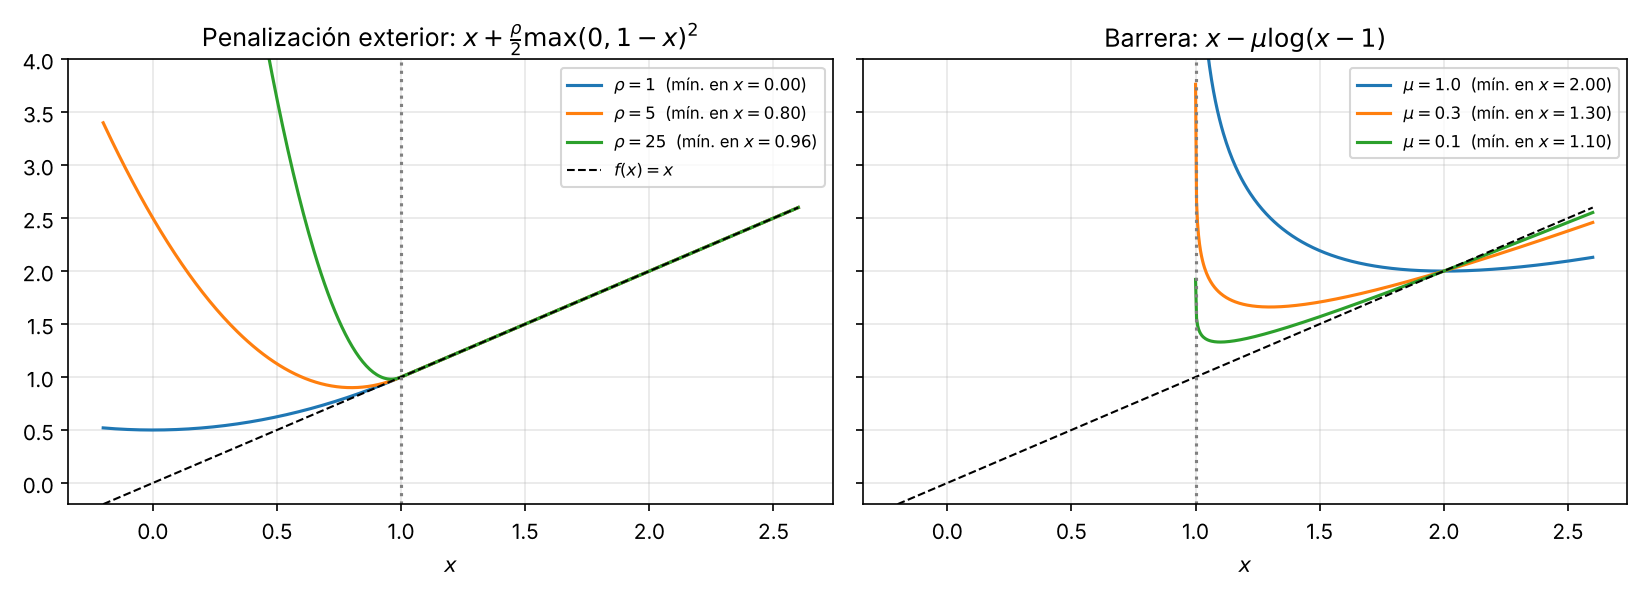
\includegraphics[width=\linewidth]{figs/fig14_penal_barrera_1d.png}
    \end{column}
    \begin{column}{0.43\textwidth}
      \small
      \textbf{Exterior}: $Q=x+\tfrac\rho2\max\{0,1-x\}^2$.\\
      $Q'=1-\rho(1-x)=0\Rightarrow x_\rho=1-\tfrac1\rho$.\\[2pt]
      El mínimo queda \textbf{fuera} (infactible) por $1/\rho$ y converge a $x^\ast=1$ cuando $\rho\to\infty$.

      \vspace{0.2cm}
      \textbf{Barrera} (ver más adelante): $B=x-\mu\log(x-1)$.\\
      $B'=1-\tfrac{\mu}{x-1}=0\Rightarrow x_\mu=1+\mu$.\\[2pt]
      El mínimo queda \textbf{dentro} (factible) por $\mu$.
    \end{column}
  \end{columns}
\end{frame}

\begin{frame}{Penalización exterior y multiplicadores}
  \begin{columns}[T]
    \begin{column}{0.52\textwidth}
      \small
      En el mínimo $x_\rho$ de $Q$: $\ \grad f+\rho\sum_jg_j^+\grad g_j=0$.\\
      Compárese con KKT: $\ \grad f+\sum_j\mu_j\grad g_j=0$.
      \begin{alertblock}{Estimador de multiplicadores}
        \[ \hat\mu_j=\rho\max\{0,g_j(x_\rho)\},\qquad \hat\lambda_i=\rho\,h_i(x_\rho) \]
        Convergen a $\mu^\ast,\lambda^\ast$ con error $O(1/\rho)$.
      \end{alertblock}
      \begin{itemize}
        \item ``Violación $\times\rho$'' = multiplicador: \textbf{cuánto cuesta} la restricción.
        \item Gratis: no hay que resolver nada extra.
      \end{itemize}
    \end{column}
    \begin{column}{0.46\textwidth}
      \tiny\centering
      \textbf{P2 (exterior)}, $\mu^\ast=(\tfrac23,\tfrac23)$\\[3pt]
      \resizebox{\linewidth}{!}{\begin{tabular}{rrrrrrrr}\toprule
$\rho$ & $x_1$ & $x_2$ & $f$ & viol.\ & $\hat\mu_1$ & $\hat\mu_2$ & cond.\\\midrule
$10^{0}$ & 1.24594 & 1.07661 & 0.57447 & 4.8e-01 & 0.476 & 0.323 & 2.9e+00\\
$10^{1}$ & 1.04053 & 1.01917 & 0.92096 & 6.4e-02 & 0.635 & 0.597 & 3.2e+00\\
$10^{2}$ & 1.00440 & 1.00219 & 0.99122 & 6.6e-03 & 0.663 & 0.659 & 3.1e+00\\
$10^{3}$ & 1.00044 & 1.00022 & 0.99911 & 6.7e-04 & 0.666 & 0.666 & 3.1e+00\\
$10^{4}$ & 1.00004 & 1.00002 & 0.99991 & 6.7e-05 & 0.667 & 0.667 & 3.1e+00\\
$10^{5}$ & 1.00000 & 1.00000 & 0.99999 & 6.7e-06 & 0.667 & 0.667 & 3.1e+00\\
$10^{6}$ & 1.00000 & 1.00000 & 1.00000 & 6.7e-07 & 0.667 & 0.667 & 3.1e+00\\
\bottomrule\end{tabular}
}
    \end{column}
  \end{columns}
\end{frame}

\begin{frame}{El precio: mal condicionamiento cuando $\rho\to\infty$}
  \begin{columns}[T]
    \begin{column}{0.5\textwidth}
      \small
      \begin{itemize}
        \item $\grad^2Q=\grad^2f+\rho\sum_jg_j^+\,\grad^2g_j+\rho\sum_{j\ \text{activas}}\grad g_j\grad g_j^\top$.
        \item El último término tiene \textbf{rango $\le$ nº de restricciones activas} y tamaño $\propto\rho$: crea \textbf{valles muy empinados} en esas direcciones y planos en las demás.
        \item $\ \text{cond}(\grad^2Q)\sim O(\rho)$ $\Rightarrow$ Newton/BFGS se vuelven inestables o lentos para $\rho$ enorme.
      \end{itemize}
      \begin{alertblock}{Por eso se usa una sucesión}
        Con $\rho$ moderado el subproblema es fácil y da un buen $x_0$ para el siguiente: \textbf{warm start}.
      \end{alertblock}
    \end{column}
    \begin{column}{0.48\textwidth}
      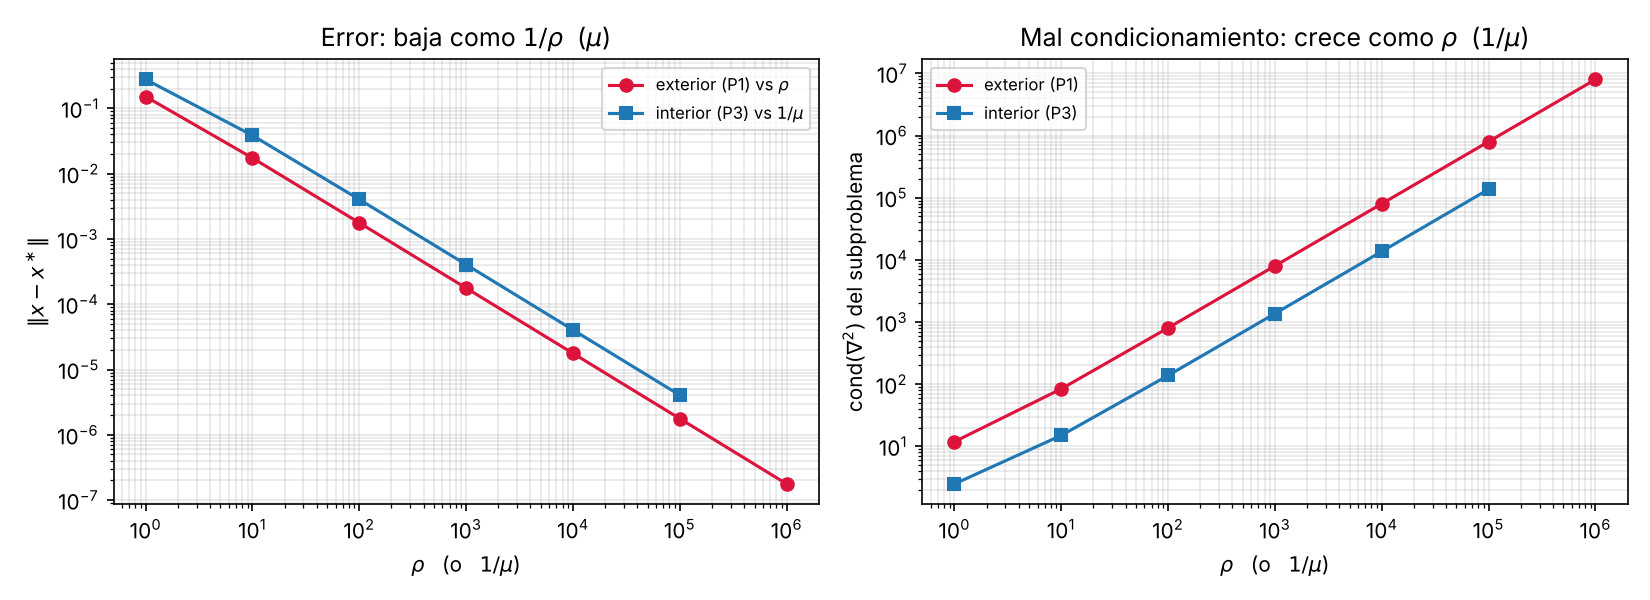
\includegraphics[width=\linewidth]{figs/fig14_error_cond.png}
    \end{column}
  \end{columns}
\end{frame}

\begin{frame}{Condicionamiento y error: P1 (exterior) y P3 (interior)}
  \centering\scriptsize
  \resizebox{0.6\linewidth}{!}{\begin{tabular}{rrrrr}\toprule
$\rho$ o $1/\mu$ & cond.\ ext.\ (P1) & cond.\ int.\ (P3) & err.\ ext.\ (P1) & err.\ int.\ (P3)\\\midrule
$10^{0}$ & 1.2e+01 & 2.5e+00 & 1.5e-01 & 2.8e-01\\
$10^{1}$ & 8.4e+01 & 1.5e+01 & 1.7e-02 & 3.8e-02\\
$10^{2}$ & 8.0e+02 & 1.4e+02 & 1.8e-03 & 4.0e-03\\
$10^{3}$ & 8.0e+03 & 1.4e+03 & 1.8e-04 & 4.0e-04\\
$10^{4}$ & 8.0e+04 & 1.4e+04 & 1.8e-05 & 4.0e-05\\
$10^{5}$ & 8.0e+05 & 1.4e+05 & 1.8e-06 & 4.0e-06\\
\bottomrule\end{tabular}
}
  \normalsize
  \vspace{0.2cm}
  \begin{itemize}
    \item \textbf{Error $\propto1/\rho$} (o $\propto\mu$): cada factor 10 en el parámetro da \textbf{un decimal} más.
    \item \textbf{Condición $\propto\rho$} (o $\propto1/\mu$): cada decimal \textbf{cuesta} un factor 10 en la condición de la Hessiana.
  \end{itemize}
  \begin{alertblock}{¿Siempre pasa?}
    No. En P2 la solución es un \textbf{vértice} (2 restricciones activas en 2 variables) y la condición \textbf{no crece} (queda en $\approx3$, tabla anterior): el mal condicionamiento aparece cuando hay \textbf{menos restricciones activas que variables}, como en P1 y P3.
  \end{alertblock}
\end{frame}

\begin{frame}{Trayectoria de la penalización exterior (P3)}
  \begin{columns}[T]
    \begin{column}{0.58\textwidth}
      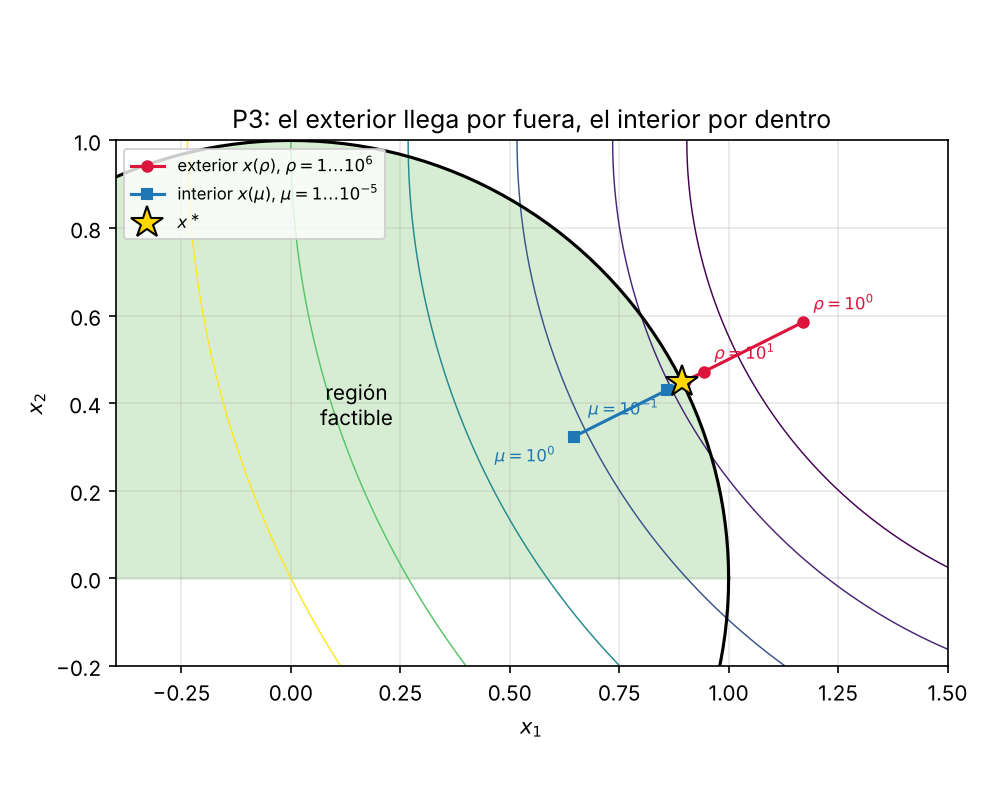
\includegraphics[width=\linewidth]{figs/fig14_trayectorias_P3.png}
    \end{column}
    \begin{column}{0.4\textwidth}
      \small
      \begin{itemize}
        \item Exterior: $x_\rho$ parte \textbf{fuera} del disco y se acerca por afuera: $\rho=1\to(1.17,0.58)$, $\rho=10\to(0.94,0.47)$, $\dots\to(0.8944,0.4472)$.
        \item Interior: $x_\mu$ parte \textbf{dentro} y se acerca por adentro.
        \item Las dos trayectorias \textbf{rodean} la solución $x^\ast$ en la frontera, una por cada lado.
        \item Estimador exterior: $\hat\mu=1.22,1.235,1.2359\to\mu^\ast=\sqrt5-1=1.2361$.
      \end{itemize}
    \end{column}
  \end{columns}
\end{frame}

\begin{frame}{Barrera interior (logarítmica)}
  \begin{block}{Función barrera (solo desigualdades $g_j\le0$)}
    \[ B(x;\mu)=f(x)-\mu\sum_j\log\bigl(-g_j(x)\bigr),\qquad \mu>0,\quad g_j(x)<0\ \text{(estrictamente factible)} \]
  \end{block}
  \begin{itemize}
    \item Si $g_j\to0^-$, entonces $-\log(-g_j)\to+\infty$: la barrera \textbf{impide} cruzar la frontera.
    \item $\mu$ grande: barrera ``gorda'', el mínimo queda lejos de la frontera (centro de la región). $\mu\to0$: la barrera se pega a la frontera y $x_\mu\to x^\ast$.
    \item Curva $\{x_\mu\}$: \textbf{camino central} (central path), base de los \textbf{métodos de punto interior}.
  \end{itemize}
  \begin{alertblock}{Requisitos}
    Necesita un punto inicial \textbf{estrictamente factible} ($g<0$) y un line search que \textbf{rechace} pasos que salgan de la región (en el código, $B=+\infty$ fuera).
  \end{alertblock}
\end{frame}

\begin{frame}{Barrera y KKT perturbadas}
  \footnotesize
  En el mínimo $x_\mu$: $\ \grad f(x_\mu)+\sum_j\dfrac{\mu}{-g_j(x_\mu)}\grad g_j(x_\mu)=0$. Definiendo
  \[ \hat\mu_j:=\frac{\mu}{-g_j(x_\mu)}>0\quad\Longrightarrow\quad
     \begin{cases}\grad f+\sum_j\hat\mu_j\grad g_j=0 &\text{(estacionariedad \checkmark{})}\\ g_j(x_\mu)<0,\ \hat\mu_j>0 &\text{(factibilidad \checkmark{})}\\ \boxed{\hat\mu_j\,g_j(x_\mu)=-\mu} &\text{(complementariedad perturbada)}\end{cases} \]
  \begin{alertblock}{Mensaje}
    La barrera resuelve las KKT con la complementariedad $\mu_jg_j=0$ \emph{relajada} a $\mu_jg_j=-\mu$. Cuando $\mu\to0$ se recupera la KKT exacta, y $\hat\mu_j\to\mu_j^\ast$.
  \end{alertblock}
  \begin{center}\tiny
  \resizebox{0.62\linewidth}{!}{\begin{tabular}{rrrrrrrr}\toprule
$\mu$ & $x_1$ & $x_2$ & $f$ & $\max g_i$ & $\hat\mu_1$ & $\hat\mu_2$ & cond.\\\midrule
$10^{0}$ & 0.47863 & 0.91189 & 2.32232 & -6.1e-01 & 1.465 & 1.641 & 1.5e+00\\
$10^{-1}$ & 0.91186 & 0.96549 & 1.18524 & -1.2e-01 & 0.746 & 0.815 & 2.2e+00\\
$10^{-2}$ & 0.99015 & 0.99523 & 1.01981 & -1.5e-02 & 0.674 & 0.684 & 3.0e+00\\
$10^{-3}$ & 0.99900 & 0.99950 & 1.00200 & -1.5e-03 & 0.667 & 0.668 & 3.1e+00\\
$10^{-4}$ & 0.99990 & 0.99995 & 1.00020 & -1.5e-04 & 0.667 & 0.667 & 3.1e+00\\
$10^{-5}$ & 0.99999 & 1.00000 & 1.00002 & -1.5e-05 & 0.667 & 0.667 & 3.1e+00\\
$10^{-6}$ & 1.00000 & 1.00000 & 1.00000 & -1.5e-06 & 0.667 & 0.667 & 3.1e+00\\
\bottomrule\end{tabular}
}\\[2pt]
  \scriptsize P2 (barrera): $\max g_i\approx-1.5\,\mu$ y $\hat\mu\to(\tfrac23,\tfrac23)$ \checkmark{}.
  \end{center}
\end{frame}

\begin{frame}{Exterior vs.\ interior}
  \centering\small
  \begin{tabular}{p{3.0cm}p{4.3cm}p{4.3cm}}
    \toprule
    & \textbf{Exterior ($\rho\uparrow$)} & \textbf{Interior ($\mu\downarrow$)}\\
    \midrule
    Iterados & \textbf{infactibles} (fuera) & \textbf{factibles} (dentro)\\
    Punto inicial & cualquiera & estrictamente factible\\
    Igualdades & sí, naturalmente & no directamente\\
    Si se detiene antes & solución infactible & solución \textbf{usable} (factible)\\
    Multiplicadores & $\rho\,g^+$ & $-\mu/g$\\
    Condicionamiento & $\sim\rho$ & $\sim1/\mu$\\
    Región factible & puede tener interior vacío & necesita interior no vacío\\
    \bottomrule
  \end{tabular}
  \vspace{0.3cm}

  \normalsize
  Las barreras con búsqueda de camino central son el origen de los \textbf{métodos de punto interior} modernos (LP, QP, NLP).
\end{frame}

\begin{frame}[fragile]{Código: el solver interno (Newton amortiguado)}
\begin{lstlisting}[basicstyle=\ttfamily\fontsize{7}{8.2}\selectfont,breaklines=false]
def newton(F, gradF, hessF, x0, tol=1e-10, max_iter=100):
    x = np.array(x0, float);  fx = F(x)
    for k in range(max_iter):
        g = gradF(x)
        if np.linalg.norm(g, np.inf) < tol:  return x
        H = hessF(x);  wmin = np.linalg.eigvalsh(H).min()
        if wmin < 1e-10:  H += (1e-6 - wmin) * np.eye(len(x))   # H > 0
        p = -np.linalg.solve(H, g);  a = 1.0
        while True:                                        # Armijo
            fn = F(x + a * p)
            if np.isfinite(fn) and fn <= fx + 1e-4*a*(g @ p) + 1e-14*(1+abs(fx)): break
            a *= 0.5
        x, fx = x + a * p, fn
    return x
\end{lstlisting}
  \footnotesize Newton con line search (Clase 4); solo cambia la función $F$ que se le pasa.
\end{frame}

\begin{frame}[fragile]{Código: $Q$ (exterior) y $B$ (interior)}
\begin{lstlisting}[basicstyle=\ttfamily\fontsize{7}{8.2}\selectfont,breaklines=false]
def penalizacion_exterior(prob, x0, rhos):
    x = np.array(x0, float)
    for rho in rhos:                                       # rho = 1, 10, ..., 1e6
        Q    = lambda x: f(x) + 0.5*rho*np.sum(np.maximum(0, g(x))**2)
        gQ   = lambda x: grad(x) + rho * Jg(x).T @ np.maximum(0, g(x))
        hQ   = lambda x: hess(x) + rho*(np.einsum("j,jab->ab", np.maximum(0,g(x)), hessg(x))
                                        + Jg(x)[g(x) > 0].T @ Jg(x)[g(x) > 0])
        x = newton(Q, gQ, hQ, x)                           # warm start: x anterior
    return x

def barrera_interior(prob, x0, mus):
    x = np.array(x0, float)                                # x0 estrictamente factible
    for mu in mus:                                         # mu = 1, 0.1, ..., 1e-5
        B  = lambda x: f(x) - mu*np.sum(np.log(-g(x))) if np.all(g(x) < 0) else np.inf
        gB = lambda x: grad(x) + mu * Jg(x).T @ (1.0 / -g(x))
        hB = lambda x: hess(x) + mu*(np.einsum("j,jab->ab", 1/-g(x), hessg(x))
                                     + Jg(x).T @ np.diag(1/g(x)**2) @ Jg(x))
        x = newton(B, gB, hB, x)
    return x
\end{lstlisting}
  \small (Versión resumida de \texttt{scripts/14\_penalizacion.py}; las Hessianas son analíticas.)
\end{frame}

\begin{frame}{Resultados en P3 y comparación con \texttt{scipy}}
  \small
  \begin{itemize}
    \item \textbf{Exterior}: 7 subproblemas ($\rho=1,\dots,10^6$), 21 iteraciones de Newton en total; error final $6\!\times\!10^{-7}$, violación $10^{-6}$ (\textbf{infactible} por construcción).
    \item \textbf{Barrera}: 6 subproblemas ($\mu=1,\dots,10^{-5}$), 38 iteraciones; error $4\!\times\!10^{-6}$, siempre factible.
    \item Comparadas con SQP (6 iteraciones, error $10^{-16}$) hacen \textbf{más trabajo} y logran \textbf{menos precisión}: pagan el mal condicionamiento y el lazo externo.
  \end{itemize}
  \begin{alertblock}{\texttt{scipy.optimize}}
    \texttt{trust-constr} usa una barrera (punto interior) para desigualdades: en P3 converge con 13 iteraciones y error $10^{-5}$ (misma precisión que nuestra barrera con $\mu_{\min}=10^{-5}$). No hay un ``método de penalización'' directo en \texttt{scipy}: es una técnica de \textbf{construcción} que se arma sobre cualquier minimizador sin restricciones, como hicimos aquí con Newton.
  \end{alertblock}
\end{frame}

\begin{frame}{Más allá: penalidad exacta y Lagrangiano aumentado}
  \small
  \begin{itemize}
    \item \textbf{Penalización $\ell_1$ exacta}: $\ f+\nu\bigl(\sum|h_i|+\sum g_j^+\bigr)$. Con $\nu>\norm{\lambda^\ast}_\infty$ el mínimo \textbf{es} $x^\ast$ con $\nu$ \textbf{finito}: sin mal condicionamiento. Costo: no es derivable (de ahí viene la función de mérito de SQP).
    \item \textbf{Lagrangiano aumentado} (método de multiplicadores):
    \[ L_A(x,\lambda;\rho)=f+\lambda^\top h+\tfrac\rho2\norm{h}^2,\qquad \lambda\leftarrow\lambda+\rho\,h(x) \]
    Con $\rho$ \textbf{moderado} y $\lambda$ actualizado converge sin $\rho\to\infty$. Es la base de ALGENCAN, LANCELOT, y de ADMM.
  \end{itemize}
  \begin{exampleblock}{Moraleja}
    El defecto de la penalización clásica ($\rho\to\infty$) se corrige \textbf{estimando bien los multiplicadores}: otra vez aparecen $\lambda,\mu$ como protagonistas.
  \end{exampleblock}
\end{frame}

\begin{frame}{Resumen de penalización y barrera}
  \begin{itemize}
    \item Penalización: problema con restricciones $\to$ \textbf{sucesión} de problemas sin restricciones; cada uno se resuelve con Newton/BFGS (Clase 4), con warm start.
    \item \textbf{Exterior}: $Q=f+\tfrac\rho2(\sum h^2+\sum g_+^2)$; iterados infactibles; $\hat\mu=\rho g^+$; error $\sim1/\rho$.
    \item \textbf{Interior}: $B=f-\mu\sum\log(-g)$; iterados factibles; $\hat\mu=-\mu/g$; KKT con complementariedad \textbf{perturbada}; error $\sim\mu$.
    \item Precio común: \textbf{condicionamiento} $\sim\rho$ o $1/\mu$ (cuando hay menos restricciones activas que variables).
    \item Simples de programar, \textbf{reusan} cualquier solver sin restricciones; pero menos eficientes que SQP cuando importa la precisión.
  \end{itemize}
\end{frame}
% ============================================================
\section{Síntesis y cierre del curso}
% ============================================================

\begin{frame}{Comparación final en P3 (convexo, óptimo en frontera curva)}
  \centering\scriptsize
  \resizebox{0.8\linewidth}{!}{\begin{tabular}{lrrrrr}\toprule
M\'etodo & iter. & eval.\ $f$ & eval.\ $\nabla f$ & $\|x-x^\ast\|$ & viol.\\\midrule
SQP (Hessiana exacta) & 6 & 19 & 13 & 0e+00 & 0e+00\\
SQP (BFGS) & 7 & 30 & 29 & 1e-16 & 0e+00\\
Cutting plane (LP) & 17 & 35 & 17 & 2e-05 & 7e-07\\
Penalización exterior & 21 & 36 & 28 & 6e-07 & 1e-06\\
Barrera interior & 38 & 52 & 44 & 4e-06 & 0e+00\\
scipy SLSQP (SQP) & 9 & 11 & 9 & 3e-15 & 0e+00\\
scipy trust-constr (barrera) & 13 & 8 & 8 & 1e-05 & 0e+00\\
\bottomrule\end{tabular}
}
  \normalsize
  \vspace{0.2cm}
  \begin{itemize}
    \item $x_0=(0.3,0.2)$ para todos. ``iter.'' = iteraciones externas (QP, LP o pasos de Newton acumulados).
    \item Las evaluaciones son \textbf{aproximadas}: cada evaluación de la función de mérito cuenta como una de $f$.
    \item La métrica relevante es el \textbf{costo para una precisión dada}; no hay un ``ganador'' universal.
  \end{itemize}
\end{frame}

\begin{frame}{Convergencia comparada (P3)}
  \begin{columns}[T]
    \begin{column}{0.6\textwidth}
      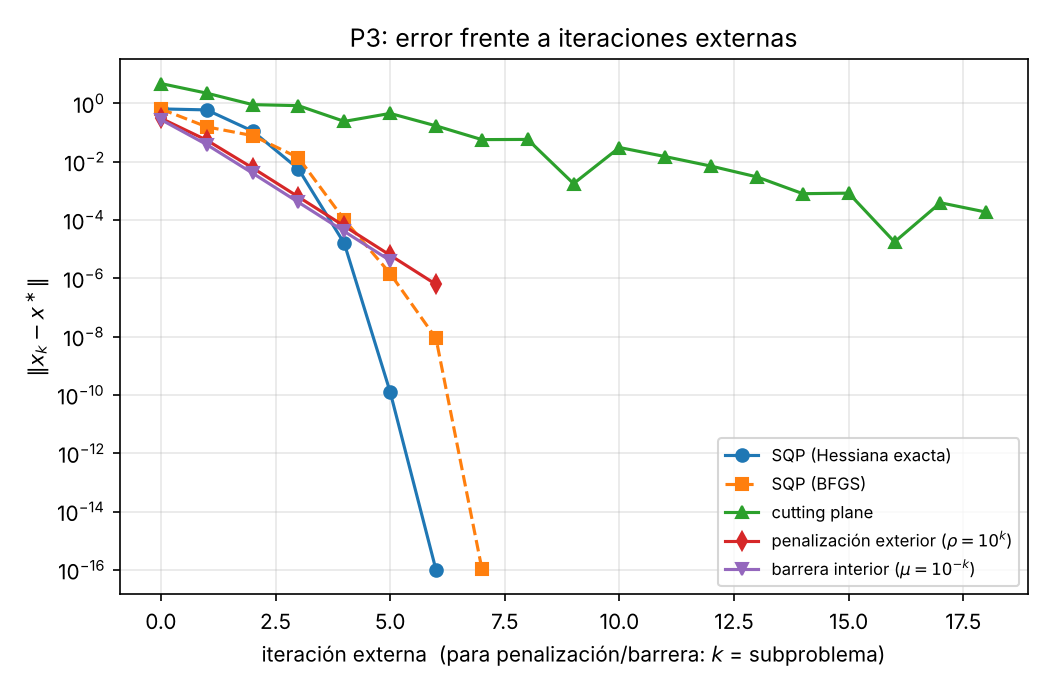
\includegraphics[width=\linewidth]{figs/fig15_comparacion_P3.png}
    \end{column}
    \begin{column}{0.38\textwidth}
      \small
      \begin{itemize}
        \item \textbf{SQP exacta}: caída superlineal/cuadrática, 6 pasos.
        \item \textbf{BFGS}: algo más lenta, sin segundas derivadas.
        \item \textbf{Cutting plane}: avance \textbf{lineal} y lento: cada corte solo mejora la aproximación poligonal.
        \item \textbf{Penalización/barrera}: error $\sim1/\rho$ o $\sim\mu$: un decimal por subproblema.
      \end{itemize}
    \end{column}
  \end{columns}
\end{frame}

\begin{frame}{P4: Rosenbrock en el disco (no convexo)}
  \centering\scriptsize
  \resizebox{0.95\linewidth}{!}{\begin{tabular}{lrrrrr}\toprule
M\'etodo & iter. & eval.\ $f$ & eval.\ $\nabla f$ & $\|x-x^\ast\|$ & viol.\\\midrule
SQP (Hessiana exacta) & 6 & 41 & 13 & 5e-09 & 0e+00\\
SQP (BFGS) & 22 & 97 & 89 & 5e-09 & 0e+00\\
Penalización exterior & 20 & 55 & 27 & 7e-08 & 1e-07\\
Barrera interior & 52 & 65 & 58 & 4e-05 & 0e+00\\
scipy SLSQP (SQP) & 17 & 23 & 17 & 5e-09 & 4e-13\\
scipy trust-constr (barrera) & 36 & 27 & 25 & 2e-07 & 0e+00\\
\bottomrule\end{tabular}
}
  \normalsize
  \vspace{0.2cm}
  \begin{itemize}
    \item $x^\ast=(0.7864,\,0.6177)$, $f^\ast=0.0457$. \textbf{Cutting plane no aplica} (la función no es convexa: los cortes no subestiman).
    \item SQP exacta y \texttt{SLSQP} llegan a $5\!\times\!10^{-9}$; la barrera sufre cerca de la frontera con la curvatura de Rosenbrock (52 iteraciones).
  \end{itemize}
\end{frame}

\begin{frame}{Visión comparada de los métodos}
  \centering\scriptsize
  \begin{tabular}{p{2.5cm}p{2.0cm}p{2.1cm}p{2.1cm}p{2.5cm}}
    \toprule
    \textbf{Método} & \textbf{Subproblema} & \textbf{Convexidad} & \textbf{Convergencia} & \textbf{Iterados}\\
    \midrule
    Cutting plane & LP & necesaria & lenta & infactibles\\
    SQP & QP & no necesaria & cuadr./superlineal & infactibles\\
    Penal.\ exterior & sin restr. & no necesaria & lineal en $\rho$ & infactibles\\
    Barrera interior & sin restr. & no necesaria & lineal en $\mu$ & factibles\\
    \bottomrule
  \end{tabular}

  \normalsize
  \vspace{0.3cm}
  \begin{itemize}
    \item \textbf{Todos} terminan en un punto que cumple las condiciones \textbf{KKT} (con las salvedades de convexidad).
    \item La diferencia está en \textbf{cómo} se aproxima el problema: lineal (CP), cuadrático (SQP), o eliminando restricciones (penalización).
  \end{itemize}
\end{frame}

\begin{frame}{Guía para elegir}
  \begin{itemize}
    \item \textbf{Pocas variables, derivadas disponibles, alta precisión} $\to$ \textbf{SQP} (\texttt{SLSQP}).
    \item \textbf{Muchas variables y restricciones, estructura dispersa} $\to$ \textbf{punto interior} (\texttt{trust-constr}, IPOPT).
    \item \textbf{Problema convexo con restricciones complicadas, se quiere cota inferior} $\to$ \textbf{cutting plane} (pensar en planos de corte, Benders).
    \item \textbf{Solo se tiene un minimizador sin restricciones} $\to$ \textbf{penalización} (preferir $\ell_1$ exacta o Lagrangiano aumentado).
    \item \textbf{Restricciones de caja} ($l\le x\le u$) $\to$ L-BFGS-B, \texttt{least\_squares(bounds=\dots)}.
  \end{itemize}
  \begin{alertblock}{Siempre}
    Verificar KKT al final y mirar los \textbf{multiplicadores}: dicen qué restricciones importan y cuánto.
  \end{alertblock}
\end{frame}

\begin{frame}{Cinco mensajes clave de la clase}
  \begin{enumerate}
    \item \textbf{KKT}: en el óptimo $-\grad f$ está en el cono de gradientes de restricciones \textbf{activas}; $\mu\ge0$, $\mu_jg_j=0$; los multiplicadores son \textbf{precios sombra}.
    \item \textbf{QP}: con restricciones lineales y objetivo cuadrático, KKT es un sistema \textbf{lineal} (igualdades) o una búsqueda del conjunto activo (desigualdades).
    \item \textbf{Cutting plane}: linearizar y resolver LPs; útil en convexos, lento por la curvatura.
    \item \textbf{SQP} = Newton sobre KKT: un QP por iteración, con el \textbf{Lagrangiano} (no solo $f$) y función de mérito.
    \item \textbf{Penalización/barrera}: eliminar restricciones a costa de \textbf{mal condicionamiento}; mejor con multiplicadores estimados (Lagrangiano aumentado).
  \end{enumerate}
\end{frame}

\begin{frame}{Conexión con todo el curso}
  \begin{columns}[T]
    \begin{column}{0.5\textwidth}
      \begin{itemize}
        \item \textbf{Sin restricciones} (Clases 1--4): gradiente, Newton, BFGS, CG, dogleg, LM.
        \item \textbf{Con restricciones} (Clase 5): se \textbf{reducen} a lo anterior: QP/LP por iteración (SQP, CP) o una sucesión de problemas libres (penalización).
      \end{itemize}
    \end{column}
    \begin{column}{0.46\textwidth}
      \begin{itemize}
        \item \textbf{Metaheurísticas} (Clase 3): no usan derivadas ni KKT; útiles cuando el problema es no diferenciable o discreto.
        \item Extensiones: gradiente conjugado con restricciones, optimización estocástica con restricciones, optimización robusta.
      \end{itemize}
    \end{column}
  \end{columns}
\end{frame}

\begin{frame}{Ejercicios propuestos}
  \small
  \begin{enumerate}
    \item Para $\min x_1^2+x_2^2$ s.a.\ $x_1+x_2\ge2$ plantee KKT y resuélvalo \textbf{a mano}. Interprete $\mu^\ast$ como precio sombra.
    \item Resuelva un QP de 3 variables con 2 desigualdades usando el método de conjunto activo; compare con \texttt{scipy}.
    \item Implemente cutting plane para $\min x_1+x_2$ s.a.\ $x_1^2+x_2^2\le1$; grafique la cota inferior $t_k$ vs.\ $f(x_k)$.
    \item En SQP use $W=\grad^2f$ en vez de $\grad^2_{xx}L$ en P3. ¿Qué ocurre? Explique.
    \item Barrera: reproduzca la tabla de $\hat\mu$ para P3 y verifique $\hat\mu_j g_j=-\mu$.
    \item Penalización exterior sobre P1: grafique la condición de la Hessiana vs.\ $\rho$ y estime la pendiente en escala log-log.
    \item (Retador) Implemente el \textbf{Lagrangiano aumentado} para P1 y compare con penalización cuadrática: ¿cuántos $\rho$ necesita?
  \end{enumerate}
\end{frame}

\begin{frame}{Referencias}
  \small
  \begin{itemize}
    \item J.\ Nocedal y S.\ Wright, \emph{Numerical Optimization}, 2.ª ed., Springer, 2006: cap.~12 (KKT), cap.~16 (QP), cap.~17 (penalización, barrera, Lagrangiano aumentado), cap.~18 (SQP).
    \item S.\ Boyd y L.\ Vandenberghe, \emph{Convex Optimization}, Cambridge, 2004: cap.~5 (dualidad, KKT), cap.~11 (puntos interiores).
    \item D.\ Bertsekas, \emph{Nonlinear Programming}, Athena Scientific, 1999.
    \item J.\ E.\ Kelley, ``The cutting-plane method for solving convex programs'', \emph{J.\ SIAM} 8(4), 1960.
    \item D.\ Kraft, ``A software package for sequential quadratic programming'', DFVLR, 1988 (\texttt{SLSQP}).
    \item Código de la clase: \texttt{scripts/10\_\dots15\_\textit{*}.py}; figuras en \texttt{figs/}.
  \end{itemize}
\end{frame}

\begin{frame}[plain]
  \centering\vfill
  {\Large\bfseries ¡Gracias!}\\[0.4cm]
  Preguntas y comentarios\vfill
\end{frame}

\end{document}
